
%% Newton Questions used on the
%% NYSED Physics Regents Examination
%%--------------------------------------------------

%% this section contains 105 problems


%% Section June2015
%%--------------------
\element{nysed}{
\begin{question}{June2015-Q04}
    A \SI{160}{\kilo\gram} space vehicle is traveling along a straight line at a constant speed of \SI{800}{\meter\per\second}. 
    The magnitude of the net force on the space vehicle is:
    \begin{multicols}{2}
    \begin{choices}
      \correctchoice{\SI{0}{\newton}}
        \wrongchoice{\SI{1.60e2}{\newton}}
        \wrongchoice{\SI{8.00e2}{\newton}}
        \wrongchoice{\SI{1.28e5}{\newton}}
    \end{choices}
    \end{multicols}
\end{question}
}

\element{nysed}{
\begin{question}{June2015-Q05}
    A student throws a \SI{5.0}{\newton} ball straight up.
    What is the net force on the ball at its maximum height?
    \begin{multicols}{2}
    \begin{choices}
        \wrongchoice{\SI{0.0}{\newton}}
        \wrongchoice{\SI{5.0}{\newton}, up}
      \correctchoice{\SI{5.0}{\newton}, down}
        \wrongchoice{\SI{9.8}{\newton}, down}
    \end{choices}
    \end{multicols}
\end{question}
}

\element{nysed}{
\begin{question}{June2015-Q07}
    A \SI{1.5}{\kilo\gram} cart initially moves at \SI{2.0}{\meter\per\second}.
    It is brought to rest by a constant net force in \SI{0.30}{\second}.
    What is the magnitude of the net force?
    \begin{multicols}{2}
    \begin{choices}
        \wrongchoice{\SI{0.40}{\newton}}
        \wrongchoice{\SI{0.90}{\newton}}
      \correctchoice{\SI{10}{\newton}}
        \wrongchoice{\SI{15}{\newton}}
    \end{choices}
    \end{multicols}
\end{question}
}

\element{nysed}{
\begin{question}{June2015-Q09}
    As a \SI{5.0e2}{\newton} basketball player jumps from the floor up toward the basket,
        the magnitude of the force of her feet on the floor is \SI{1.0e3}{\newton}.
    As she jumps, the magnitude of the force of the floor on her feet is:
    \begin{multicols}{2}
    \begin{choices}
        \wrongchoice{\SI{5.0e2}{\newton}}
      \correctchoice{\SI{1.0e3}{\newton}}
        \wrongchoice{\SI{1.5e3}{\newton}}
        \wrongchoice{\SI{5.0e5}{\newton}}
    \end{choices}
    \end{multicols}
\end{question}
}

\element{nysed}{
\begin{question}{June2015-Q33}
    A different force is applied to each of four different blocks on a frictionless, horizontal surface. 
    In which diagram does the block have the greatest inertia \SI{2.0}{\second} after starting from rest?
    \begin{multicols}{2}
    \begin{choices}
        \AMCboxDimensions{down=-0.20cm}
        \correctchoice{
            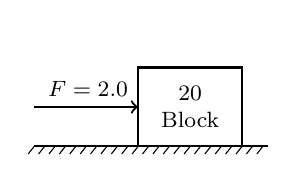
\begin{tikzpicture}[font=\footnotesize,xscale=0.66]
                \draw[white] (-2.0,1.5) -- (2.0,1.5);
                %% Force
                \draw[thick,->] (-2,0.5) -- (0,0.5)
                    node[pos=1.0,anchor=south east] {$F=\SI{2.0}{\newton}$};
                %% Block
                \draw[thick] (0,0) rectangle (2,1);
                \node[anchor=center,text width=3em,text centered]
                    at (1,0.5) {\SI{20}{\kilo\gram} Block};
                %% Floor
                \draw[thick] (-2,0) -- (2.5,0);
                \foreach \x in {-20,-18,...,25}
                    \draw[thin] (\x mm,0cm) -- ++ (220:0.15cm);
            \end{tikzpicture}
        }
        \wrongchoice{
            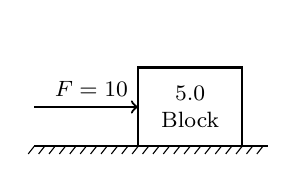
\begin{tikzpicture}[font=\footnotesize,xscale=0.66]
                \draw[white] (-2.0,1.5) -- (2.0,1.5);
                %% Force
                \draw[thick,->] (-2,0.5) -- (0,0.5)
                    node[pos=1.0,anchor=south east] {$F=\SI{10}{\newton}$};
                %% Block
                \draw[thick] (0,0) rectangle (2,1);
                \node[anchor=center,text width=3em,text centered]
                    at (1,0.5) {\SI{5.0}{\kilo\gram} Block};
                %% Floor
                \draw[thick] (-2,0) -- (2.5,0);
                \foreach \x in {-20,-18,...,25}
                    \draw[thin] (\x mm,0cm) -- ++ (220:0.15cm);
            \end{tikzpicture}
        }
        \wrongchoice{
            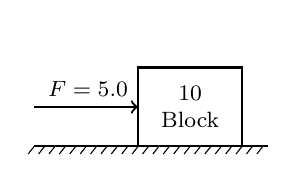
\begin{tikzpicture}[font=\footnotesize,xscale=0.66]
                \draw[white] (-2.0,1.5) -- (2.0,1.5);
                %% Force
                \draw[thick,->] (-2,0.5) -- (0,0.5)
                    node[pos=1.0,anchor=south east] {$F=\SI{5.0}{\newton}$};
                %% Block
                \draw[thick] (0,0) rectangle (2,1);
                \draw[thick] (0,0) rectangle (2,1);
                \node[anchor=center,text width=3em,text centered]
                    at (1,0.5) {\SI{10}{\kilo\gram} Block};
                %% Floor
                \draw[thick] (-2,0) -- (2.5,0);
                \foreach \x in {-20,-18,...,25}
                    \draw[thin] (\x mm,0cm) -- ++ (220:0.15cm);
            \end{tikzpicture}
        }
        \wrongchoice{
            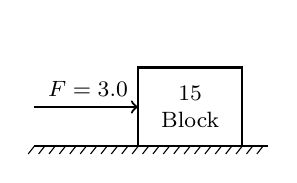
\begin{tikzpicture}[font=\footnotesize,xscale=0.66]
                \draw[white] (-2.0,1.5) -- (2.0,1.5);
                %% Force
                \draw[thick,->] (-2,0.5) -- (0,0.5)
                    node[pos=1.0,anchor=south east] {$F=\SI{3.0}{\newton}$};
                %% Block
                \draw[thick] (0,0) rectangle (2,1);
                \node[anchor=center,text width=3em,text centered]
                    at (1,0.5) {\SI{15}{\kilo\gram} Block};
                %% Floor
                \draw[thick] (-2,0) -- (2.5,0);
                \foreach \x in {-20,-18,...,25}
                    \draw[thin] (\x mm,0cm) -- ++ (220:0.15cm);
            \end{tikzpicture}
        }
    \end{choices}
    \end{multicols}
\end{question}
}

\element{nysed}{
\begin{question}{June2015-Q41}
    An object is in equilibrium. 
    Which force vector diagram could represent the force(s) acting on the object?
    \begin{multicols}{2}
    \begin{choices}
        \AMCboxDimensions{down=-1.3cm}
        \wrongchoice{
            \begin{tikzpicture}
                \draw[white] (-1.00,-1.5) rectangle (1.00,1.0);
                \node[draw,fill=white!90!black,circle,inner sep=0pt,minimum size=8pt] (A) at (0,0) {};
                \draw[thick,->] (A) -- ++ (270:1.414cm);
            \end{tikzpicture}
        }
        \wrongchoice{
            \begin{tikzpicture}
                \draw[white] (-1.00,-1.5) rectangle (1.00,1.0);
                \node[draw,fill=white!90!black,circle,inner sep=0pt,minimum size=8pt] (A) at (0,0) {};
                \draw[thick,->] (A) -- ++ (270:1.414cm);
                \draw[thick,->] (A) -- ++ (90:0.707cm);
            \end{tikzpicture}
        }
        \wrongchoice{
            \begin{tikzpicture}
                \draw[white] (-1.00,-1.5) rectangle (1.00,1.0);
                \node[draw,fill=white!90!black,circle,inner sep=0pt,minimum size=8pt] (A) at (0,0) {};
                \draw[thick,->] (A) -- ++ (0:0.707cm);
                \draw[thick,->] (A) -- ++ (180:0.707cm);
                \draw[thick,->] (A) -- ++ (270:1.414cm);
            \end{tikzpicture}
        }
        \correctchoice{
            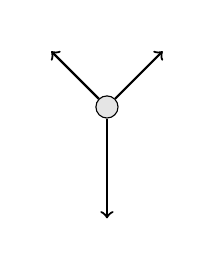
\begin{tikzpicture}
                \draw[white] (-1.00,-1.5) rectangle (1.00,1.0);
                \node[draw,fill=white!90!black,circle,inner sep=0pt,minimum size=8pt] (A) at (0,0) {};
                \draw[thick,->] (A) -- ++ (45:1.00cm);
                \draw[thick,->] (A) -- ++ (135:1.00cm);
                \draw[thick,->] (A) -- ++ (270:1.414cm);
            \end{tikzpicture}
        }
    \end{choices}
    \end{multicols}
\end{question}
}


%% Section June2014
%%--------------------
\element{nysed}{
\begin{question}{June2014-Q05}
    A baseball bat exerts a force of magnitude $F$ on a ball.
    If the mass of the bat is three times the mass of the ball,
        the magnitude of the force of the ball on the bat is:
    \begin{multicols}{2}
    \begin{choices}
      \correctchoice{$F$}
        \wrongchoice{$2F$}
        \wrongchoice{$3F$}
        \wrongchoice{$F/3$}
    \end{choices}
    \end{multicols}
\end{question}
}

\element{nysed}{
\begin{question}{June2014-Q08}
    A \SI{750}{\newton} person stands in an elevator that is accelerating downward.
    The upward force of the elevator floor on the person must be:
    \begin{choices}
      \correctchoice{less than \SI{750}{\newton}}
        \wrongchoice{equal to \SI{0}{\newton}}
        \wrongchoice{equal to \SI{750}{\newton}}
        \wrongchoice{greater than \SI{750}{\newton}}
    \end{choices}
\end{question}
}


%% Section June2013
%%--------------------
\element{nysed}{
\begin{question}{June2013-Q09}
    Which situation represents a person in equilibrium?
    \begin{choices}
        \wrongchoice{a child gaining speed while sliding a slide}
        \wrongchoice{a woman accelerating upward in an elevator}
      \correctchoice{a man standing on a bathroom scale}
        \wrongchoice{a teenager driving around a corner in his car}
    \end{choices}
\end{question}
}

\element{nysed}{
\begin{question}{June2013-Q10}
    A rock is thrown straight up into the air.
    At the highest point of the rock's path,
        the magnitude of the net force acting on the rock is:
    \begin{choices}
        \wrongchoice{less than the magnitude of the rock's weight, but greater than zero}
        \wrongchoice{greater than the magnitude of the rock's weight}
      \correctchoice{the same as the magnitude of the rock's weight}
        \wrongchoice{zero}
    \end{choices}
\end{question}
}

\element{nysed}{
\begin{question}{June2013-Q11}
    The diagram below shows a compressed spring between two carts initially at rest on a horizontal frictionless surface.
    Cart $A$ has a mass of \SI{2.0}{\kilo\gram} and cart $B$ has a mass of \SI{1.0}{\kilo\gram}.
    A string holds the carts together.
    \begin{center}
    \begin{tikzpicture}
        %% Ground
        \node[anchor=north,fill,pattern=north east lines,minimum width=8cm, minimum height=0.05cm] at (0,0) {};
        \draw (-4,0) -- (4,0);
        %% carts
        \node[draw,minimum width=2cm,minimum height=2em,anchor=south] (A) at (-2,0.3) {\SI{2}{\kilo\gram}};
        \node[draw,minimum width=1cm,minimum height=2em,anchor=south] (B) at (2,0.3) {\SI{1}{\kilo\gram}};
        \node[anchor=south] at (A.north) {$A$};
        \node[anchor=south] at (B.north) {$B$};
        %% wheels
        \draw[fill=white!90!black] (A.south west) ++(0:0.2cm) arc(90:-270:0.15);
        \draw[fill=white!90!black] (A.south east) ++(180:0.2cm) arc(90:-270:0.15);
        \draw[fill=white!90!black] (B.south west) ++(0:0.2cm) arc(90:-270:0.15);
        \draw[fill=white!90!black] (B.south east) ++(180:0.2cm) arc(90:-270:0.15);
        %% Spring
        \draw[decoration={aspect=0.2,segment length=1.5mm,amplitude=2mm,coil},decorate] (A.east) -- (B.west);
        \draw[thick] (A.north east) -- (B.north west);
    \end{tikzpicture}
    \end{center}
    The string is cut and the carts move apart.
    Compared to the magnitude of the force the spring exerts on cart $A$,
        the magnitude of the force the spring exerts on cart $B$ is:
    \begin{choices}
      \correctchoice{the same}
        \wrongchoice{half as great}
        \wrongchoice{twice as great}
        \wrongchoice{four times as great}
    \end{choices}
\end{question}
}

\element{nysed}{
\begin{question}{June2013-Q38}
    Four forces act concurrently on a block on a horizontal surface as shown in the diagram below.
    \begin{center}
    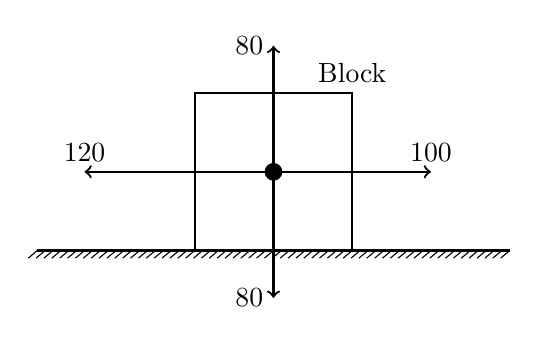
\begin{tikzpicture}
        \draw[fill] (0,0) circle (3pt);
        \draw[thick,->] (0,0) -- (0:2cm)
            node[anchor=south] {\SI{100}{\newton}};
        \draw[thick,->] (0,0) -- (90:1.6cm)
            node[anchor=east] {\SI{80}{\newton}};
        \draw[thick,->] (0,0) -- (180:2.4cm)
            node[anchor=south] {\SI{120}{\newton}};
        \draw[thick,->] (0,0) -- (270:1.6cm)
            node[anchor=east] {\SI{80}{\newton}};
        \draw[thick] (-1,-1) rectangle (1,1)
            node[anchor=south] {Block};
        \draw[thick] (-3,-1) -- (3,-1);
        \foreach \x in {-30,-29,...,30}
            \draw[thin] (\x mm,-1cm) -- ++ (220:0.15cm);
    \end{tikzpicture}
    \end{center}
    As a result of these forces, the block:
    \begin{choices}
        \wrongchoice{moves at constant speed to the right}
        \wrongchoice{moves at constant speed to the left}
        \wrongchoice{accelerates to the right}
      \correctchoice{accelerates to the left}
    \end{choices}
\end{question}
}

\element{nysed}{
\begin{question}{June2013-Q40}
    A \SI{4.0}{\kilo\gram} object is accelerated at \SI{3.0}{\meter\per\second\squared} north by an unbalanced force.
    The same unbalanced force acting on a \SI{2.0}{\kilo\gram} object will accelerate this object toward the north at:
    \begin{multicols}{2}
    \begin{choices}
        \wrongchoice{\SI{12}{\meter\per\second\squared}}
      \correctchoice{\SI{6.0}{\meter\per\second\squared}}
        \wrongchoice{\SI{3.0}{\meter\per\second\squared}}
        \wrongchoice{\SI{1.5}{\meter\per\second\squared}}
    \end{choices}
    \end{multicols}
\end{question}
}


%% Section June2012
%%--------------------
\element{nysed}{
\begin{question}{June2012-Q07}
    Which situation describes an object that has \emph{no} unbalanced force acting on it?
    \begin{choices}
        \wrongchoice{an apple in free fall}
        \wrongchoice{a satellite orbiting Earth}
      \correctchoice{a hockey puck moving at constant velocity}
        \wrongchoice{a laboratory cart moving down a frictionless \ang{30} incline}
    \end{choices}
\end{question}
}

\element{nysed}{
\begin{question}{June2012-Q12}
    A number of \SI{1.0}{\newton} horizontal forces are exerted on a block on a frictionless, horizontal surface.
    Which top-view diagram shows the forces producing the greatest magnitude of acceleration of the block?
    \begin{multicols}{2}
    \begin{choices}
        \AMCboxDimensions{down=-1.0cm}
        \correctchoice{
            \begin{tikzpicture}[font=\footnotesize]
                \draw[white] (-1.6,-1.6) rectangle (1.6,1.6);
                \node[draw,rectangle,minimum size=1cm,text centered,text width=1cm]
                    (B) at (0,0) {Top of Block};
                \draw[thick,->] (B.east) -- ++(0:1cm)
                    node[pos=0.5,anchor=south] {\SI{1.0}{\newton}};
                \draw[thick,->] (B.south) -- ++(270:1cm)
                    node[pos=0.5,anchor=east] {\SI{1.0}{\newton}};
            \end{tikzpicture}
        }
        \wrongchoice{
            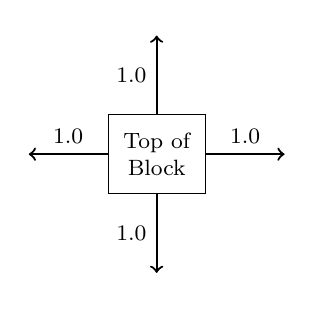
\begin{tikzpicture}[font=\footnotesize]
                \draw[white] (-1.6,-1.6) rectangle (1.6,1.6);
                \node[draw,rectangle,minimum size=1cm,text centered,text width=1cm]
                    (B) at (0,0) {Top of Block};
                \draw[thick,->] (B.north) -- ++(90:1cm)
                    node[pos=0.5,anchor=east] {\SI{1.0}{\newton}};
                \draw[thick,->] (B.east) -- ++(0:1cm)
                    node[pos=0.5,anchor=south] {\SI{1.0}{\newton}};
                \draw[thick,->] (B.south) -- ++(270:1cm)
                    node[pos=0.5,anchor=east] {\SI{1.0}{\newton}};
                \draw[thick,->] (B.west) -- ++(180:1cm)
                    node[pos=0.5,anchor=south] {\SI{1.0}{\newton}};
            \end{tikzpicture}
        }
        \wrongchoice{
            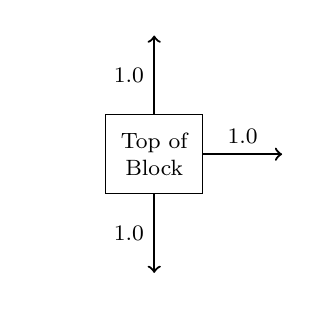
\begin{tikzpicture}[font=\footnotesize]
                \draw[white] (-1.6,-1.6) rectangle (1.6,1.6);
                \node[draw,rectangle,minimum size=1cm,text centered,text width=1cm]
                    (B) at (0,0) {Top of Block};
                \draw[thick,->] (B.north) -- ++(90:1cm)
                    node[pos=0.5,anchor=east] {\SI{1.0}{\newton}};
                \draw[thick,->] (B.east) -- ++(0:1cm)
                    node[pos=0.5,anchor=south] {\SI{1.0}{\newton}};
                \draw[thick,->] (B.south) -- ++(270:1cm)
                    node[pos=0.5,anchor=east] {\SI{1.0}{\newton}};
            \end{tikzpicture}
        }
        \wrongchoice{
            \begin{tikzpicture}[font=\footnotesize]
                \draw[white] (-1.6,-1.6) rectangle (1.6,1.6);
                \node[draw,rectangle,minimum size=1cm,text centered,text width=1cm]
                    (B) at (0,0) {Top of Block};
                \draw[thick,->] (B.north) -- ++(90:1cm)
                    node[pos=0.5,anchor=east] {\SI{1.0}{\newton}};
                \draw[thick,->] (B.south) -- ++(270:1cm)
                    node[pos=0.5,anchor=east] {\SI{1.0}{\newton}};
            \end{tikzpicture}
        }
    \end{choices}
    \end{multicols}
\end{question}
}

%% NOTE: June2012-Q47 is too big


%% Section June2011
%%--------------------
\element{nysed}{
\begin{question}{June2011-Q06}
    A student is standing in an elevator that is accelerating downward.
    The force that the student exerts on the floor of the elevator must be:
    \begin{choices}
      \correctchoice{less than the weight of the student when at rest}
        \wrongchoice{greater than the weight of the student when at rest}
        \wrongchoice{less than the force of the floor on the student}
        \wrongchoice{greater than the force of the floor on the student}
    \end{choices}
\end{question}
}

\element{nysed}{
\begin{question}{June2011-Q12}
    Two forces act concurrently on an object on a horizontal,
        frictionless surface, as shown in the diagram below.
    \begin{center}
    \begin{tikzpicture}
        %% Ground
        \node[anchor=north,fill,pattern=north east lines,minimum width=8cm, minimum height=0.05cm] at (0,0) {};
        \draw (-4,0) -- (4,0);
        \node at (0,-0.5) {Horizontal, frictionless surface.};
        %% Object
        \node[draw,minimum size=1.6cm,anchor=south] (A) at (0,0) {Object};
        %% Forces
        \draw[thick,->] (A.west) -- ++(180:2) node[pos=0.5,anchor=south] {\SI{10}{\newton}};
        \draw[thick,->] (A.east) -- ++(0:1.2) node[pos=0.5,anchor=south] {\SI{6}{\newton}};
    \end{tikzpicture}
    \end{center}
    What additional force, when applied to the object,
        will establish equilibrium?
    \begin{choices}
        \wrongchoice{\SI{16}{\newton} toward the right}
        \wrongchoice{\SI{16}{\newton} toward the left}
        \wrongchoice{\SI{4}{\newton} toward the right}
      \correctchoice{\SI{4}{\newton} toward the left}
    \end{choices}
\end{question}
}

\element{nysed}{
\begin{question}{June2011-Q38}
    A \SI{75}{\kilo\gram} hockey player is skating across the ice at a speed of \SI{6.0}{\meter\per\second}.
    What is the magnitude of the average force required to stop the player in \SI{0.65}{\second}?
    \begin{multicols}{2}
    \begin{choices}
        \wrongchoice{\SI{120}{\newton}}
        \wrongchoice{\SI{290}{\newton}}
      \correctchoice{\SI{690}{\newton}}
        \wrongchoice{\SI{920}{\newton}}
    \end{choices}
    \end{multicols}
\end{question}
}


%% Section June2010
%%--------------------
\element{nysed}{
\begin{question}{June2010-Q04}
    A \SI{0.149}{\kilo\gram} baseball,
        initially moving at \SI{15}{\meter\per\second},
        is brought to rest in \SI{0.040}{\second} by a baseball glove on a catcher's hand.
    The magnitude of the average force exerted on the ball by the glove is:
    \begin{multicols}{2}
    \begin{choices}
        \wrongchoice{\SI{2.2}{\newton}}
        \wrongchoice{\SI{2.9}{\newton}}
        \wrongchoice{\SI{17}{\newton}}
      \correctchoice{\SI{56}{\newton}}
    \end{choices}
    \end{multicols}
\end{question}
}

\element{nysed}{
\begin{question}{June2010-Q05}
    Which body is in equilibrium?
    \begin{choices}
        \wrongchoice{A satellite moving around Earth in a circular orbit.}
        \wrongchoice{A cart rolling down a frictionless incline.}
        \wrongchoice{An apple falling freely toward the surface of Earth.}
      \correctchoice{A block sliding at constant velocity across a tabletop.}
    \end{choices}
\end{question}
}

\element{nysed}{
\begin{question}{June2010-Q08}
    A student pulls a \SI{60}{\newton} sled with a force having a magnitude of \SI{20}{\newton}.
    What is the magnitude of the force that the sled exerts on the student?
    \begin{multicols}{2}
    \begin{choices}
      \correctchoice{\SI{20}{\newton}}
        \wrongchoice{\SI{40}{\newton}}
        \wrongchoice{\SI{60}{\newton}}
        \wrongchoice{\SI{80}{\newton}}
    \end{choices}
    \end{multicols}
\end{question}
}

\element{nysed}{
\begin{question}{June2010-Q10}
    The diagram below shows a horizontal \SI{12}{\newton} force being applied to two blocks, $A$ and $B$, initially at rest on a horizontal, frictionless surface.
    Block $A$ has a mass of \SI{1.0}{\kilo\gram} and block $B$ has a mass of \SI{2.0}{\kilo\gram}.
    \begin{center}
    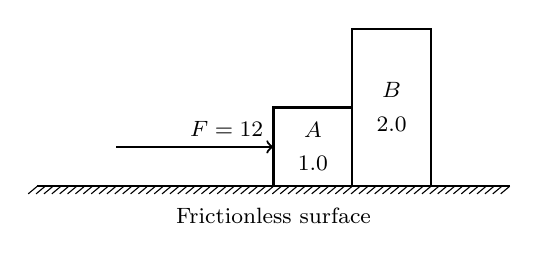
\begin{tikzpicture}[font=\footnotesize]
        %% Force
        \draw[thick,->] (-2,0.5) -- (0,0.5)
            node[above left] {$F=\SI{12}{\newton}$};
        %% Block A
        \draw[thick] (0,0) rectangle (1,1);
        \node[anchor=south] at (0.5,0.5) {$A$};
        \node[anchor=north] at (0.5,0.5) {\SI{1.0}{\kilo\gram}};
        %% Block B
        \draw[thick] (1,0) rectangle (2,2);
        \node[anchor=south] at (1.5,1) {$B$};
        \node[anchor=north] at (1.5,1) {\SI{2.0}{\kilo\gram}};
        %% Floor
        \draw[thick] (-3,0) -- (3,0);
        \foreach \x in {-30,-29,...,30}
            \draw[thin] (\x mm,0cm) -- ++ (220:0.15cm);
        \node[anchor=north] at (0,-0.15) {Frictionless surface};
    \end{tikzpicture}
    \end{center}
    The magnitude of the acceleration of block $B$ is:
    \begin{multicols}{2}
    \begin{choices}
        \wrongchoice{\SI{6.0}{\meter\per\second\squared}}
        \wrongchoice{\SI{2.0}{\meter\per\second\squared}}
        \wrongchoice{\SI{3.0}{\meter\per\second\squared}}
      \correctchoice{\SI{4.0}{\meter\per\second\squared}}
    \end{choices}
    \end{multicols}
\end{question}
}


%% Section June2009
%%--------------------
\element{nysed}{
\begin{question}{June2009-Q05}
    A \SI{25}{\newton} weight falls freely from rest from the roof of a building.
    What is the total distance the weight falls in the first \SI{1.0}{\second}?
    \begin{multicols}{2}
    \begin{choices}
        \wrongchoice{\SI{19.6}{\meter}}
        \wrongchoice{\SI{9.8}{\meter}}
      \correctchoice{\SI{4.9}{\meter}}
        \wrongchoice{\SI{2.5}{\meter}}
    \end{choices}
    \end{multicols}
\end{question}
}

\element{nysed}{
\begin{question}{June2009-Q09}
    A \SI{0.50}{\kilo\gram} cart is rolling at a speed of \SI{0.40}{\meter\per\second}.
    If the speed of the cart is doubled, the inertia of the cart is:
    \begin{multicols}{2}
    \begin{choices}
        \wrongchoice{halved}
        \wrongchoice{doubled}
        \wrongchoice{quadrupled}
      \correctchoice{unchanged}
    \end{choices}
    \end{multicols}
\end{question}
}

\element{nysed}{
\begin{question}{June2009-Q10}
    Two forces, $F_1$ and $F_2$, are applied to a block on a frictionless,
        horizontal surface as shown below.
    \begin{center}
    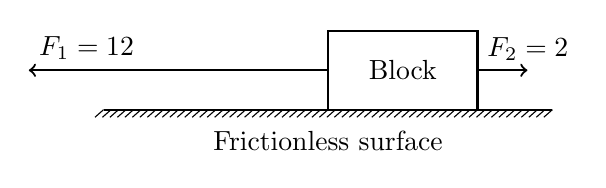
\begin{tikzpicture}[xscale=0.95]
        %% Force 1
        \draw[thick,->] (0,0.5) -- (-4,0.5)
            node[above right] {$F_1=\SI{12}{\newton}$};
        %% Force 2
        \draw[thick,->] (2,0.5) -- (2.667,0.5);
        \node[anchor=south west] at (2,0.5) {$F_2=\SI{2}{\newton}$};
        %% Block
        \draw[thick] (0,0) rectangle (2,1);
        \node[anchor=center] at (1,0.5) {Block};
        %% Floor
        \draw[thick] (-3,0) -- (3,0);
        \foreach \x in {-30,-29,...,30}
            \draw[thin] (\x mm,0cm) -- ++ (220:0.15cm);
        \node[anchor=north] at (0,-0.15) {Frictionless surface};
    \end{tikzpicture}
    \end{center}
    If the magnitude of the block's acceleration is \SI{2.0}{\meter\per\second\squared},
        what is the mass of the block?
    \begin{multicols}{2}
    \begin{choices}
        \wrongchoice{\SI{1}{\kilo\gram}}
      \correctchoice{\SI{5}{\kilo\gram}}
        \wrongchoice{\SI{6}{\kilo\gram}}
        \wrongchoice{\SI{7}{\kilo\gram}}
    \end{choices}
    \end{multicols}
\end{question}
}

\element{nysed}{
\begin{question}{June2009-Q12}
    What is the weight of a \SI{2.00}{\kilo\gram} object on the surface of Earth?
    \begin{multicols}{2}
    \begin{choices}
        \wrongchoice{\SI{4.91}{\newton}}
        \wrongchoice{\SI{2.00}{\newton}}
        \wrongchoice{\SI{9.81}{\newton}}
      \correctchoice{\SI{19.6}{\newton}}
    \end{choices}
    \end{multicols}
\end{question}
}

\element{nysed}{
\begin{question}{June2009-Q40}
    A motorcycle being driven on a dirt path hits a rock.
    Its \SI{60}{\kilo\gram} cyclist is project over the handlebars at \SI{20}{\meter\per\second} into a haystack.
    If the cyclist is brought to rest in \SI{0.50}{\second},
        the magnitude of the average force exerted on the cyclist by haystack is:
    \begin{multicols}{2}
    \begin{choices}
        \wrongchoice{\SI{6.0e1}{\newton}}
        \wrongchoice{\SI{5.9e2}{\newton}}
        \wrongchoice{\SI{1.2e3}{\newton}}
      \correctchoice{\SI{2.4e3}{\newton}}
    \end{choices}
    \end{multicols}
\end{question}
}


%% Section Jan2009
%%--------------------
\element{nysed}{
\begin{question}{Jan2009-Q01}
    A force of \SI{25}{\newton} east and a force of \SI{25}{\newton} west act concurrently on a \SI{5.0}{\kilo\gram} cart.
    What is the acceleration of the cart?
    \begin{multicols}{2}
    \begin{choices}
        \wrongchoice{\SI{1.0}{\meter\per\second\squared} west}
        \wrongchoice{\SI{0.20}{\meter\per\second\squared} east}
        \wrongchoice{\SI{5.0}{\meter\per\second\squared} east}
      \correctchoice{\SI{0}{\meter\per\second\squared}}
    \end{choices}
    \end{multicols}
\end{question}
}

\element{nysed}{
\begin{question}{Jan2009-Q03}
    What is the acceleration due to gravity at a location where a \SI{15.0}{\kilo\gram} mass weighs \SI{45.0}{\newton}?
    \begin{multicols}{2}
    \begin{choices}
        \wrongchoice{\SI{675}{\meter\per\second\squared}}
        \wrongchoice{\SI{9.81}{\meter\per\second\squared}}
      \correctchoice{\SI{3.0}{\meter\per\second\squared}}
        \wrongchoice{\SI{0.333}{\meter\per\second\squared}}
    \end{choices}
    \end{multicols}
\end{question}
}

\element{nysed}{
\begin{question}{Jan2009-Q38}
    Which graph best represents the motion of an object in equilibrium?
    \begin{multicols}{2}
    \begin{choices}
        \AMCboxDimensions{down=-2.5em}
        \correctchoice{
            \begin{tikzpicture}
                \begin{axis}[
                    axis y line=left,
                    axis x line=bottom,
                    axis line style={->},
                    xlabel={time},
                    xtick=\empty,
                    ylabel={displacement},
                    ytick=\empty,
                    xmin=0,xmax=11,
                    ymin=0,ymax=11,
                    width=1.0\columnwidth,
                ]
                \addplot[line width=1pt,domain=0:10]{x};
                \end{axis}
            \end{tikzpicture}
        }
        \wrongchoice{
            \begin{tikzpicture}
                \begin{axis}[
                    axis y line=left,
                    axis x line=bottom,
                    axis line style={->},
                    xlabel={time},
                    xtick=\empty,
                    ylabel={velocity},
                    ytick=\empty,
                    xmin=0,xmax=11,
                    ymin=0,ymax=11,
                    width=1.0\columnwidth,
                ]
                \addplot[line width=1pt,domain=0:10]{x};
                \end{axis}
            \end{tikzpicture}
        }
        \wrongchoice{
            \begin{tikzpicture}
                \begin{axis}[
                    axis y line=left,
                    axis x line=bottom,
                    axis line style={->},
                    xlabel={time},
                    xtick=\empty,
                    ylabel={displacement},
                    ytick=\empty,
                    xmin=0,xmax=11,
                    ymin=0,ymax=11,
                    width=1.0\columnwidth,
                ]
                \addplot[line width=1pt,domain=0:10]{0.1*x*x};
                \end{axis}
            \end{tikzpicture}
        }
        \wrongchoice{
            \begin{tikzpicture}
                \begin{axis}[
                    axis y line=left,
                    axis x line=bottom,
                    axis line style={->},
                    xlabel={time},
                    xtick=\empty,
                    ylabel={velocity},
                    ytick=\empty,
                    xmin=0,xmax=11,
                    ymin=0,ymax=11,
                    width=1.0\columnwidth,
                ]
                \addplot[line width=1pt,domain=0:10]{0.1*x*x};
                \end{axis}
            \end{tikzpicture}
        }
    \end{choices}
    \end{multicols}
\end{question}
}


%% Section Aug2008
%%--------------------
\element{nysed}{
\begin{question}{Aug2008-Q01}
    A net force of \SI{25}{\newton} is applied horizontally to a \SI{10}{\kilo\gram} block resting on a table.
    What is the magnitude of the acceleration of the block?
    \begin{multicols}{2}
    \begin{choices}
        \wrongchoice{\SI{0.0}{\meter\per\second\squared}}
        \wrongchoice{\SI{0.26}{\meter\per\second\squared}}
        \wrongchoice{\SI{0.40}{\meter\per\second\squared}}
      \correctchoice{\SI{2.5}{\meter\per\second\squared}}
    \end{choices}
    \end{multicols}
\end{question}
}

\element{nysed}{
\begin{question}{Aug2008-Q06}
    If the magnitude of the gravitational force of Earth on the Moon is $F$,
        the magnitude of the gravitational force of the Moon on Earth is:
    \begin{choices}
        \wrongchoice{smaller than $F$}
        \wrongchoice{larger than $F$}
      \correctchoice{equal to $F$}
    \end{choices}
\end{question}
}

\element{nysed}{
\begin{question}{Aug2008-Q07}
    Which term represents a scalar quantity?
    \begin{multicols}{2}
    \begin{choices}
      \correctchoice{distance}
        \wrongchoice{displacement}
        \wrongchoice{force}
        \wrongchoice{weight}
    \end{choices}
    \end{multicols}
\end{question}
}


%% Section June2008
%%--------------------
\element{nysed}{
\begin{question}{June2008-Q09}
    Which diagram represents a box in equilibrium?
    \begin{multicols}{2}
    \begin{choices}
        \AMCboxDimensions{down=-1.5cm}
        \wrongchoice{
            \begin{tikzpicture}
                \draw[draw=white] (-1.6,-1.6) rectangle (1.6,1.6);
                \node[draw,rectangle,minimum size=2em] (B) at (0,0) {Box};
                \draw[thick,<-] (B.east) -- ++(0:1.15cm) node[pos=0.5,anchor=south] {\SI{5}{\newton}};
                \draw[thick,<-] (B.west) -- ++(180:1.15cm) node[pos=0.5,anchor=south] {\SI{5}{\newton}};
                \draw[thick,->] (B.south) -- ++(270:1.15cm) node[pos=0.5,anchor=west] {\SI{5}{\newton}};
            \end{tikzpicture}
        }
        \correctchoice{
            \begin{tikzpicture}
                \draw[draw=white] (-1.6,-1.6) rectangle (1.6,1.6);
                \node[draw,rectangle,minimum size=2em] (B) at (0,0) {Box};
                \draw[thick,->] (B.north) -- ++(90:0.5cm) node[pos=1.0,anchor=south] {\SI{2}{\newton}};
                \draw[thick,->] (B.south) -- ++(270:0.5cm) node[pos=1.0,anchor=north] {\SI{2}{\newton}};
                \draw[thick,<-] (B.west) -- ++(180:1.15cm) node[pos=0.5,anchor=south] {\SI{5}{\newton}};
                \draw[thick,<-] (B.east) -- ++(0:1.15cm) node[pos=0.5,anchor=south] {\SI{5}{\newton}};
            \end{tikzpicture}
        }
        \wrongchoice{
            \begin{tikzpicture}
                \draw[draw=white] (-1.6,-1.6) rectangle (1.6,1.6);
                \node[draw,rectangle,minimum size=2em] (B) at (0,0) {Box};
                \draw[thick,<-] (B.west) -- ++(180:0.5cm) node[pos=1.0,anchor=east] {\SI{2}{\newton}};
                \draw[thick,<-] (B.east) -- ++(0:0.5cm) node[pos=1.0,anchor=west] {\SI{2}{\newton}};
                \draw[thick,->] (B.north) -- ++(90:0.5cm) node[pos=1.0,anchor=south] {\SI{2}{\newton}};
                \draw[thick,->] (B.south) -- ++(270:1.15cm) node[pos=0.5,anchor=west] {\SI{5}{\newton}};
            \end{tikzpicture}
        }
        \wrongchoice{
            \begin{tikzpicture}
                \draw[draw=white] (-1.6,-1.6) rectangle (1.6,1.6);
                \node[draw,rectangle,minimum size=2em] (B) at (0,0) {Box};
                \draw[thick,<-] (B.east) -- ++(0:0.72cm) node[pos=0.5,anchor=south west] {\SI{3}{\newton}};
                \draw[thick,<-] (B.south) -- ++(270:0.5cm) node[pos=1.0,anchor=north] {\SI{2}{\newton}};
                \draw[thick,<-] (B.west) -- ++(180:1.15cm) node[pos=0.5,anchor=south] {\SI{5}{\newton}};
            \end{tikzpicture}
        }
    \end{choices}
    \end{multicols}
\end{question}
}

\element{nysed}{
\begin{question}{June2008-Q15}
    A carpenter hits a nail with a hammer.
    Compared to the magnitude of the force the hammer exerts on the nail,
        the magnitude of the force the nail exerts on the hammer during contact is:
    \begin{choices}
        \wrongchoice{less}
        \wrongchoice{greater}
      \correctchoice{the same}
    \end{choices}
\end{question}
}

\element{nysed}{
\begin{question}{June2008-Q40}
    A \SI{25}{\newton} horizontal force northward and a \SI{35}{\newton} horizontal force southward act concurrently on a \SI{15}{\kilo\gram} object on a frictionless surface.
    What is the magnitude of the object's acceleration?
    \begin{multicols}{2}
    \begin{choices}
      \correctchoice{\SI{0.67}{\meter\per\second\squared}}
        \wrongchoice{\SI{1.7}{\meter\per\second\squared}}
        \wrongchoice{\SI{2.3}{\meter\per\second\squared}}
        \wrongchoice{\SI{4.0}{\meter\per\second\squared}}
    \end{choices}
    \end{multicols}
\end{question}
}


%% Section Jan2008
%%--------------------
\element{nysed}{
\begin{question}{Jan2008-Q12}
    If a \SI{65}{\kilo\gram} astronaut exerts a force with a magnitude of \SI{50}{\newton} on a satellite that she is repairing,
        the magnitude of the force that the satellite exerts on her is:
    \begin{choices}
        \wrongchoice{\SI{0}{\newton}}
        \wrongchoice{\SI{50}{\newton} less than her weight}
        \wrongchoice{\SI{50}{\newton} more than her weight}
      \correctchoice{\SI{50}{\newton}}
    \end{choices}
\end{question}
}

\element{nysed}{
\begin{question}{Jan2008-Q39}
    A bicycle and its rider have a combined mass of \SI{80}{\kilo\gram} and a speed of \SI{6.0}{\meter\per\second}.
    What is the magnitude of the average force needed to bring the bicycle and its rider to a stop in \SI{4.0}{\second}?
    \begin{multicols}{2}
    \begin{choices}
      \correctchoice{\SI{1.2e2}{\newton}}
        \wrongchoice{\SI{3.2e2}{\newton}}
        \wrongchoice{\SI{4.8e2}{\newton}}
        \wrongchoice{\SI{1.9e3}{\newton}}
    \end{choices}
    \end{multicols}
\end{question}
}


%% Section June2007
%%--------------------
\element{nysed}{
\begin{question}{June2007-Q03}
    A \SI{2.00}{\kilo\gram} object weighs \SI{19.6}{\newton} on Earth.
    If the acceleration due to gravity on Mars is \SI{3.71}{\meter\per\second\squared},
        what is the object's mass on Mars?
    \begin{multicols}{2}
    \begin{choices}
        \wrongchoice{\SI{2.64}{\kilo\gram}}
        \wrongchoice{\SI{19.6}{\newton}}
      \correctchoice{\SI{2.00}{\kilo\gram}}
        \wrongchoice{\SI{7.42}{\newton}}
    \end{choices}
    \end{multicols}
\end{question}
}

\element{nysed}{
\begin{question}{June2007-Q37}
    A force of \SI{1}{\newton} is equivalent to:
    \begin{multicols}{2}
    \begin{choices}
      \correctchoice{\SI{1}{\kilo\gram\meter\per\second\squared}}
        \wrongchoice{\SI{1}{\kilo\gram\meter\per\second}}
        \wrongchoice{\SI{1}{\kilo\gram\meter\squared\per\second}}
        \wrongchoice{\SI{1}{\kilo\gram\squared\meter\squared\per\second\squared}}
    \end{choices}
    \end{multicols}
\end{question}
}


%% Section Jan2007
%%--------------------
\element{nysed}{
\begin{question}{Jan2007-Q11}
    A \SI{0.15}{\kilo\gram} baseball moving at \SI{20}{\meter\per\second} is stopped by a catcher in \SI{0.010}{\second}.
    The average force stopping the ball is:
    \begin{multicols}{2}
    \begin{choices}
      \correctchoice{\SI{3.0e1}{\newton}}
        \wrongchoice{\SI{3.0e0}{\newton}}
        \wrongchoice{\SI{3.0e-2}{\newton}}
        \wrongchoice{\SI{3.0e2}{\newton}}
    \end{choices}
    \end{multicols}
\end{question}
}


%% Section June2006
%%--------------------
\element{nysed}{
\begin{question}{June2006-Q09}
    A \SI{60}{\kilo\gram} student jumps down from a laboratory counter.
    At the instant he lands on the floor his speed is \SI{3}{\meter\per\second}.
    If the student stops in \SI{0.2}{\second},
        what is the average force on the student?
    \begin{multicols}{2}
    \begin{choices}
      \correctchoice{\SI{9e2}{\newton}}
        \wrongchoice{\SI{1e-2}{\newton}}
        \wrongchoice{\SI{1e2}{\newton}}
        \wrongchoice{\SI{4}{\newton}}
    \end{choices}
    \end{multicols}
\end{question}
}

\element{nysed}{
\begin{question}{June2006-Q37}
    A \SI{2.0}{\kilo\gram} object is falling freely near Earth's surface.
    %% What is the magnitude of the gravitational force that Earth exerts on the object?
    %% NOTE: I prefer this wording
    What is the magnitude of the gravitational force that the \SI{2.0}{\kilo\gram} object exerts on Earth?
    \begin{multicols}{2}
    \begin{choices}
      \correctchoice{\SI{20.}{\newton}}
        \wrongchoice{\SI{2.0}{\newton}}
        \wrongchoice{\SI{0.20}{\newton}}
        \wrongchoice{\SI{0.0}{\newton}}
    \end{choices}
    \end{multicols}
\end{question}
}


%% Section Jan2006
%%--------------------
\element{nysed}{
\begin{question}{Jan2006-Q05}
    A \SI{2.0}{\kilo\gram} laboratory cart is sliding across a horizontal frictionless surface at a constant velocity of \SI{4.0}{\meter\per\second} east.
    What will be the cart's velocity after a \SI{6.0}{\newton} westward force acts on it for \SI{2.0}{\second}?
    \begin{multicols}{2}
    \begin{choices}
      \correctchoice{\SI{2.0}{\meter\per\second} west}
        \wrongchoice{\SI{2.0}{\meter\per\second} east}
        \wrongchoice{\SI{10.}{\meter\per\second} west}
        \wrongchoice{\SI{10.}{\meter\per\second} east}
    \end{choices}
    \end{multicols}
\end{question}
}

\newcommand{\nysedJanTwentyZeroSixQSeven}{
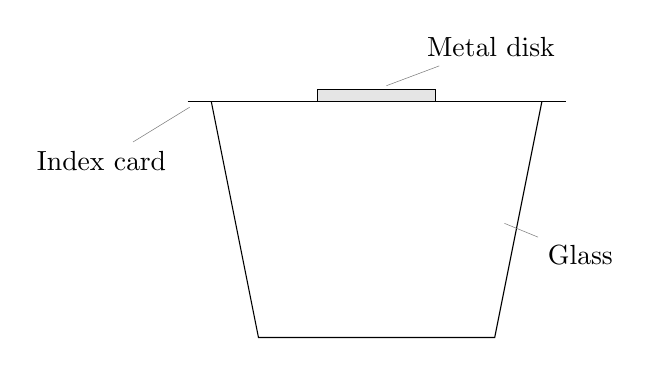
\begin{tikzpicture}[scale=0.75]
    %% glass and index card
    \draw (-3.2,0) -- (3.2,0);
    \draw (-2.8,0) -- (-2,-4) -- (2,-4) -- (2.8,0);
    %% megal disk
    \draw[fill=white!90!black] (-1,0) rectangle (1,0.2);
    %% labels
    \node[pin={30:Metal disk}] at (0,0.2) {};
    \node[pin={240:Index card}] at (-3,0) {};
    \node[pin={340:Glass}] at (2.0,-2) {};
\end{tikzpicture}
}

\element{nysed}{
\begin{question}{Jan2006-Q07}
    The diagram below shows a \SI{1.0}{\newton} metal disk resting on an index card that is balanced on top of a glass.
    \begin{center}
        \nysedJanTwentyZeroSixQSeven
    \end{center}
    What is the net force acting on the disk?
    \begin{multicols}{2}
    \begin{choices}
      \correctchoice{\SI{0}{\newton}}
        \wrongchoice{\SI{1.0}{\newton}}
        \wrongchoice{\SI{2.0}{\newton}}
        \wrongchoice{\SI{9.8}{\newton}}
    \end{choices}
    \end{multicols}
\end{question}
}

\element{nysed}{
\begin{question}{Jan2006-Q08}
    The diagram below shows a \SI{1.0}{\newton} metal disk resting on an index card that is balanced on top of a glass.
    \begin{center}
        \nysedJanTwentyZeroSixQSeven
    \end{center}
    When the index card is quickly pulled away from the glass in a horizontal direction,
        the disk falls straight down into the glass.
    This action is a result of the disk's
    \begin{multicols}{2}
    \begin{choices}
        \wrongchoice{inertia}
        \wrongchoice{charge}
        \wrongchoice{shape}
        \wrongchoice{temperature}
    \end{choices}
    \end{multicols}
\end{question}
}

\element{nysed}{
\begin{question}{Jan2006-Q11}
    A \SI{400}{\newton} girl standing on a dock exerts a force of \SI{100}{\newton} on a \SI{10000}{\newton} sailboat as she pushes is away from the dock.
    How much force does the sailboat exert on the girl?
    \begin{multicols}{2}
    \begin{choices}
      \correctchoice{\SI{100}{\newton}}
        \wrongchoice{\SI{25}{\newton}}
        \wrongchoice{\SI{400}{\newton}}
        \wrongchoice{\SI{10000}{\newton}}
    \end{choices}
    \end{multicols}
\end{question}
}


%% Section June2005
%%--------------------
\element{nysed}{
\begin{question}{June2005-Q01}
    A \SI{2.0}{\kilo\gram} body is initially traveling at a velocity of \SI{40}{\meter\per\second} east.
    If a constant force of \SI{10}{\newton} due east is applied to the body for \SI{5.0}{\second},
        the final speed of the body is:
    \begin{multicols}{2}
    \begin{choices}
      \correctchoice{\SI{65}{\meter\per\second}}
        \wrongchoice{\SI{130}{\meter\per\second}}
        \wrongchoice{\SI{15}{\meter\per\second}}
        \wrongchoice{\SI{25}{\meter\per\second}}
    \end{choices}
    \end{multicols}
\end{question}
}

\element{nysed}{
\begin{question}{June2005-Q09}
    A container of rocks with a mass of \SI{65.0}{\kilo\gram} is brought back from the moon's surface where the acceleration of gravity is \SI{1.62}{\meter\per\second\squared}.
    What is the weight of the container of rocks on Earth's surface?
    \begin{multicols}{2}
    \begin{choices}
      \correctchoice{\SI{638}{\newton}}
        \wrongchoice{\SI{394}{\newton}}
        \wrongchoice{\SI{105}{\newton}}
        \wrongchoice{\SI{65.0}{\newton}}
    \end{choices}
    \end{multicols}
\end{question}
}


%% Section Jan2005
%%--------------------
\element{nysed}{
\begin{question}{Jan2005-Q07}
    Two carts are pushed apart by an expanding spring,
        as shown in the diagram below.
    \begin{center}
    \begin{tikzpicture}
        %% Ground
        \node[anchor=north,fill,pattern=north east lines,minimum width=8cm, minimum height=0.05cm] at (0,0) {};
        \draw (-4,0) -- (4,0);
        %% Carts
        \node[draw,minimum height=0.8cm,minimum width=1.2cm,anchor=south] (L) at (-1.8,0.2) {\SI{1}{\kilo\gram}};
        \node[draw,minimum height=0.8cm,minimum width=1.8cm,anchor=south] (R) at (+1.8,0.2) {\SI{2}{\kilo\gram}};
        \draw[fill=white] (L.south west) ++(0:0.3) circle (0.2);
        \draw[fill=white] (L.south east) ++(180:0.3) circle (0.2);
        \draw[fill=white] (R.south west) ++(0:0.4) circle (0.2);
        \draw[fill=white] (R.south east) ++(180:0.4) circle (0.2);
        %% Spring
        \draw[decoration={aspect=0.2,segment length=1.5mm,amplitude=2mm,coil},decorate] (L.east) -- (R.west);
        %% Forces
        \draw[very thick,->] (L.west) -- ++(180:1cm);
        \draw[very thick,->] (R.east) -- ++(0:1cm);
    \end{tikzpicture}
    \end{center}
    If the average force on the \SI{1}{\kilo\gram} cart is \SI{1}{\newton},
        what is the average force on the \SI{2}{\kilo\gram} cart?
    \begin{multicols}{2}
    \begin{choices}
      \correctchoice{\SI{1}{\newton}}
        \wrongchoice{\SI{0.0}{\newton}}
        \wrongchoice{\SI{0.5}{\newton}}
        \wrongchoice{\SI{4}{\newton}}
    \end{choices}
    \end{multicols}
\end{question}
}


%% Section June2004
%%--------------------
\element{nysed}{
\begin{question}{June2004-Q03}
    A person is standing on a bathroom scale in an elevator car.
    If the scale reads a value greater than the weight of the person at rest,
        the elevator car could be moving:
    \begin{choices}
      \correctchoice{upward at increasing speed}
        \wrongchoice{upward at constant speed}
        \wrongchoice{downward at increasing speed}
        \wrongchoice{downward at constant speed}
    \end{choices}
\end{question}
}

\element{nysed}{
\begin{question}{June2004-Q10}
    A man is pushing a baby stroller.
    Compared to the magnitude of the force exerted on the stroller by a the man,
        the magnitude of the force exerted on the man by the stroller is:
    \begin{choices}
        \wrongchoice{zero}
        \wrongchoice{smaller, but greater than zero}
        \wrongchoice{larger}
      \correctchoice{the same}
    \end{choices}
\end{question}
}

\element{nysed}{
\begin{question}{June2004-Q36}
    A constant unbalanced force is applied to an object for a period of time.
    Which graph best represents the acceleration of the object as a function of elapsed time?
    \begin{multicols}{2}
    \begin{choices}
        \AMCboxDimensions{down=-2.5em}
        \correctchoice{
            \begin{tikzpicture}
                \begin{axis}[
                    axis y line=left,
                    axis x line=bottom,
                    axis line style={->},
                    xlabel={time},
                    xtick=\empty,
                    ylabel={acceleration},
                    ytick=\empty,
                    xmin=0,xmax=11,
                    ymin=0,ymax=11,
                    width=1.0\columnwidth,
                ]
                \addplot[line width=1pt,domain=0:10]{8};
                \end{axis}
            \end{tikzpicture}
        }
        \wrongchoice{
            \begin{tikzpicture}
                \begin{axis}[
                    axis y line=left,
                    axis x line=bottom,
                    axis line style={->},
                    xlabel={time},
                    xtick=\empty,
                    ylabel={acceleration},
                    ytick=\empty,
                    xmin=0,xmax=11,
                    ymin=0,ymax=11,
                    width=1.0\columnwidth,
                ]
                \addplot[line width=1pt,domain=0:10]{10-x};
                \end{axis}
            \end{tikzpicture}
        }
        \wrongchoice{
            \begin{tikzpicture}
                \begin{axis}[
                    axis y line=left,
                    axis x line=bottom,
                    axis line style={->},
                    xlabel={time},
                    xtick=\empty,
                    ylabel={acceleration},
                    ytick=\empty,
                    xmin=0,xmax=11,
                    ymin=0,ymax=11,
                    width=1.0\columnwidth,
                ]
                \addplot[line width=1pt,domain=0:10]{x};
                \end{axis}
            \end{tikzpicture}
        }
        \wrongchoice{
            \begin{tikzpicture}
                \begin{axis}[
                    axis y line=left,
                    axis x line=bottom,
                    axis line style={->},
                    xlabel={time},
                    xtick=\empty,
                    ylabel={acceleration},
                    ytick=\empty,
                    xmin=0,xmax=11,
                    ymin=0,ymax=11,
                    width=1.0\columnwidth,
                ]
                \addplot[line width=1pt,domain=0:10]{0.1*x*x};
                \end{axis}
            \end{tikzpicture}
        }
    \end{choices}
    \end{multicols}
\end{question}
}


%% Section Jan2004
%%--------------------
\element{nysed}{
\begin{question}{Jan2004-Q11}
    A \SI{40.}{\kilo\gram} mass is moving across a horizontal surface at \SI{4.0}{\meter\per\second}.
    What is the magnitude of the net force required to bring the mass to a stop in \SI{8.0}{\second}?
    \begin{multicols}{2}
    \begin{choices}
      \correctchoice{\SI{25}{\newton}}
        \wrongchoice{\SI{1.0}{\newton}}
        \wrongchoice{\SI{5.0}{\newton}}
        \wrongchoice{\SI{40.}{\newton}}
    \end{choices}
    \end{multicols}
\end{question}
}

\element{nysed}{
\begin{question}{Jan2004-Q38}
    A high school physics student is sitting in a seat reading this question.
        The magnitude of the force with which the seat is pushing up on the student to support him is closest to
    \begin{multicols}{2}
    \begin{choices}
      \correctchoice{\SI{600}{\newton}}
        \wrongchoice{\SI{0}{\newton}}
        \wrongchoice{\SI{60}{\newton}}
        \wrongchoice{\SI{6000}{\newton}}
        %% Added by jphafner
        %\wrongchoice{\SI{60000}{\newton}}
        %\wrongchoice{\SI{600000}{\newton}}
    \end{choices}
    \end{multicols}
\end{question}
}


%% Section June2003
%%--------------------
\element{nysed}{
\begin{question}{June2003-Q05}
    A man standing on a scale in an elevator notices that the scale reads \SI{30}{\newton} greater than his normal weight.
    Which type of movement of the elevator could cause this greater-than-normal reading?
    \begin{choices}
      \correctchoice{accelerating upward}
        \wrongchoice{accelerating downward}
        \wrongchoice{moving upward at constant speed}
        \wrongchoice{moving downward at constant speed}
    \end{choices}
\end{question}
}

\element{nysed}{
\begin{question}{June2003-Q08}
    A \SI{60}{\kilo\gram} skydiver is falling at a constant speed near the surface of Earth.
    The magnitude of the force of air friction acting on the skydiver is approximately:
    \begin{multicols}{2}
    \begin{choices}
      \correctchoice{\SI{600}{\newton}}
        \wrongchoice{\SI{60}{\newton}}
        \wrongchoice{\SI{6}{\newton}}
        \wrongchoice{\SI{0}{\newton}}
    \end{choices}
    \end{multicols}
\end{question}
}

\element{nysed}{
\begin{question}{June2003-Q11}
    When a \SI{12}{\newton} horizontal force is applied to a box on a horizontal tabletop, the box remains at rest.
    The force of static friction acting on the box is:
    \begin{choices}
        \wrongchoice{\SI{0}{\newton}}
        \wrongchoice{between \SI{0}{\newton} and \SI{12}{\newton}}
      \correctchoice{\SI{12}{\newton}}
        \wrongchoice{greater than \SI{12}{\newton}}
    \end{choices}
\end{question}
}

\element{nysed}{
\begin{question}{June2003-Q13}
    A \SI{1.5}{\kilo\gram} lab cart is accelerated uniformly from rest to a speed of \SI{2.0}{\meter\per\second} in \SI{0.5}{\second}.
    What is the magnitude of the force producing this acceleration?
    \begin{multicols}{2}
    \begin{choices}
      \correctchoice{\SI{6.0}{\newton}}
        \wrongchoice{\SI{3.0}{\newton}}
        \wrongchoice{\SI{0.70}{\newton}}
        \wrongchoice{\SI{1.5}{\newton}}
    \end{choices}
    \end{multicols}
\end{question}
}

\element{nysed}{
\begin{question}{June2003-Q46}
    Which graph best represents the motion of an object that is \emph{not} in equilibrium as it travels along a straight line?
    \begin{multicols}{2}
    \begin{choices}
        \AMCboxDimensions{down=-2.5em}
        \correctchoice{
            \begin{tikzpicture}
                \begin{axis}[
                    axis y line=left,
                    axis x line=bottom,
                    axis line style={->},
                    xlabel={time},
                    xtick=\empty,
                    ylabel={speed},
                    ytick=\empty,
                    xmin=0,xmax=11,
                    ymin=0,ymax=11,
                    width=1.0\columnwidth,
                ]
                \addplot[line width=1pt,domain=0:10]{x};
                \end{axis}
            \end{tikzpicture}
        }
        \wrongchoice{
            \begin{tikzpicture}
                \begin{axis}[
                    axis y line=left,
                    axis x line=bottom,
                    axis line style={->},
                    xlabel={time},
                    xtick=\empty,
                    ylabel={distance},
                    ytick=\empty,
                    xmin=0,xmax=11,
                    ymin=0,ymax=11,
                    width=1.0\columnwidth,
                ]
                \addplot[line width=1pt,domain=0:10]{x};
                \end{axis}
            \end{tikzpicture}
        }
        \wrongchoice{
            \begin{tikzpicture}
                \begin{axis}[
                    axis y line=left,
                    axis x line=bottom,
                    axis line style={->},
                    xlabel={time},
                    xtick=\empty,
                    ylabel={speed},
                    ytick=\empty,
                    xmin=0,xmax=11,
                    ymin=0,ymax=11,
                    width=1.0\columnwidth,
                ]
                \addplot[line width=1pt,domain=0:10]{8};
                \end{axis}
            \end{tikzpicture}
        }
        \wrongchoice{
            \begin{tikzpicture}
                \begin{axis}[
                    axis y line=left,
                    axis x line=bottom,
                    axis line style={->},
                    xlabel={time},
                    xtick=\empty,
                    ylabel={distance},
                    ytick=\empty,
                    xmin=0,xmax=11,
                    ymin=0,ymax=11,
                    width=1.0\columnwidth,
                ]
                \addplot[line width=1pt,domain=0:10]{8};
                \end{axis}
            \end{tikzpicture}
        }
    \end{choices}
    \end{multicols}
\end{question}
}


%% Section Jan2003
%%--------------------
\element{nysed}{
\begin{question}{Jan2003-Q01}
    The diagram below shows a worker using a rope to pull a car.
    \begin{center}
        %% too complex to tikz
        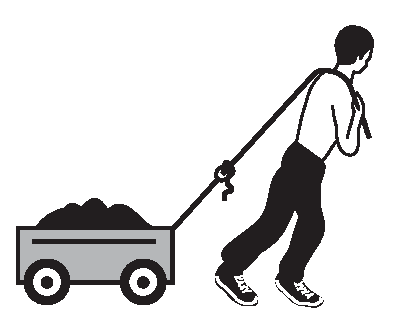
\includegraphics[keepaspectratio,scale=0.75]{Jan2003-Q01}
    \end{center}
    The worker's pull on the handle of the cart can best be described as a force having:
    \begin{choices}
      \correctchoice{both magnitude and direction}
        \wrongchoice{magnitude, only}
        \wrongchoice{direction, only}
        \wrongchoice{neither magnitude nor direction}
    \end{choices}
\end{question}
}

\element{nysed}{
\begin{question}{Jan2003-Q04}
    The sum of all forces acting on a moving object is zero,
        the object will:
    \begin{choices}
      \correctchoice{continue moving with constant velocity}
        \wrongchoice{slow down and stop}
        \wrongchoice{change the direction of its motion}
        \wrongchoice{accelerate uniformly}
    \end{choices}
\end{question}
}

\element{nysed}{
\begin{question}{Jan2003-Q05}
    A net force of \SI{10}{\newton} accelerates an object at \SI{5.0}{\meter\per\second\squared}.
    What net force would be required to accelerate the same object at \SI{1.0}{\meter\per\second\squared}?
    \begin{multicols}{2}
    \begin{choices}
      \correctchoice{\SI{2.0}{\newton}}
        \wrongchoice{\SI{1.0}{\newton}}
        \wrongchoice{\SI{5.0}{\newton}}
        \wrongchoice{\SI{50}{\newton}}
    \end{choices}
    \end{multicols}
\end{question}
}

\element{nysed}{
\begin{question}{Jan2003-Q07}
    A \SI{1200}{\kilo\gram} car traveling at \SI{10}{\meter\per\second} hits a tree and is brought to rest in \SI{0.10}{\second}.
    What is the magnitude of the average force acting on the car to bring it to rest?
    \begin{multicols}{2}
    \begin{choices}
      \correctchoice{\SI{1.2e5}{\newton}}
        \wrongchoice{\SI{1.2e4}{\newton}}
        \wrongchoice{\SI{1.2e3}{\newton}}
        \wrongchoice{\SI{1.2e2}{\newton}}
    \end{choices}
    \end{multicols}
\end{question}
}

\element{nysed}{
\begin{question}{Jan2003-Q08}
    A spring scale reads \SI{20}{\newton} as it pulls a \SI{5.0}{\kilo\gram} mass across a table.
    What is the magnitude of the force exerted by the mass on the spring scale?
    \begin{multicols}{2}
    \begin{choices}
      \correctchoice{\SI{20}{\newton}}
        \wrongchoice{\SI{49}{\newton}}
        \wrongchoice{\SI{3.0}{\newton}}
        \wrongchoice{\SI{4.0}{\newton}}
    \end{choices}
    \end{multicols}
\end{question}
}

\element{nysed}{
\begin{question}{Jan2003-Q37}
    The diagram below shows a force of magnitude $F$ applied to a mass at angle $\theta$ relative to a horizontal frictionless surface.
    \begin{center}
    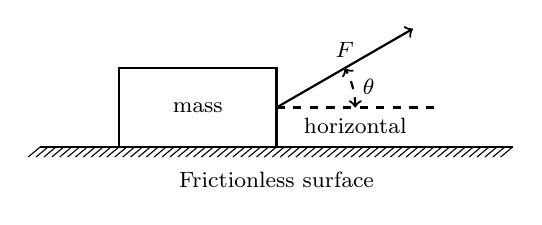
\begin{tikzpicture}[font=\footnotesize]
        %% Block
        \draw[thick] (-2,0) rectangle (0,1);
        \node[anchor=center] at (-1.0,0.5) {mass};
        %% Force 1
        \draw[dashed,thick] (0,0.5) -- (2.00,0.5)
            node[pos=0.5,anchor=north] {horizontal};
        \draw[thick,->] (0,0.5) -- ++(30:2)
            node[pos=0.5,anchor=south] {$F$};
        \draw[thick,dashed,<->] (1.0,0.5) arc (0:30:1.0)
            node[pos=0.5,anchor=west] {$\theta$};
        %% Floor
        \draw[thick] (-3,0) -- (3,0);
        \foreach \x in {-30,-29,...,30}
            \draw[thin] (\x mm,0cm) -- ++ (220:0.20cm);
        \node[anchor=north] at (0,-0.20) {Frictionless surface};
    \end{tikzpicture}
    \end{center}
    As angle $\theta$ is increased, the horizontal acceleration of the mass:
    \begin{choices}
      \correctchoice{decreases}
        \wrongchoice{increases}
        \wrongchoice{remains the same}
    \end{choices}
\end{question}
}


%% Section Aug2002
%%--------------------
\element{nysed}{
\begin{question}{Aug2002-Q01}
    A net force of \SI{25}{\newton} is applied horizontally to a \SI{10}{\kilo\gram} block resting on a table.
    What is the magnitude of the acceleration of the block?
    \begin{multicols}{2}
    \begin{choices}
        \wrongchoice{\SI{0.0}{\meter\per\second\squared}}
        \wrongchoice{\SI{0.26}{\meter\per\second\squared}}
        \wrongchoice{\SI{0.40}{\meter\per\second\squared}}
      \correctchoice{\SI{2.5}{\meter\per\second\squared}}
    \end{choices}
    \end{multicols}
\end{question}
}

\element{nysed}{
\begin{question}{Aug2002-Q06}
    If the magnitude of the gravitational force of Earth on the Moon is $F$,
        the magnitude of the gravitational force of the Moon on Earth is:
    \begin{choices}
        \wrongchoice{smaller than $F$}
        \wrongchoice{larger than $F$}
      \correctchoice{equal to $F$}
    \end{choices}
\end{question}
}

\element{nysed}{
\begin{question}{Aug2002-Q27}
    During a collision, an \SI{84}{\kilo\gram} driver of a car moving at \SI{24}{\meter\per\second} is brought to rest by an inflating air bag in \SI{1.2}{\second}.
    The magnitude of the force exerted on the driver by the air bag is approximately:
    \begin{multicols}{2}
    \begin{choices}
        \wrongchoice{\SI{7.0e1}{\newton}}
        \wrongchoice{\SI{8.2e2}{\newton}}
      \correctchoice{\SI{1.7e3}{\newton}}
        \wrongchoice{\SI{2.0e3}{\newton}}
    \end{choices}
    \end{multicols}
\end{question}
}

\element{nysed}{
\begin{question}{Aug2002-Q28}
    An apple weighing \SI{1}{\newton} on the surface of Earth has a mass of approximately:
    \begin{multicols}{2}
    \begin{choices}
      \correctchoice{\SI{e-1}{\kilo\gram}}
        \wrongchoice{\SI{e0}{\kilo\gram}}
        \wrongchoice{\SI{e1}{\kilo\gram}}
        \wrongchoice{\SI{e2}{\kilo\gram}}
    \end{choices}
    \end{multicols}
\end{question}
}

\element{nysed}{
\begin{question}{Aug2002-Q31}
    In which situation is the net force on the object equal to zero?
    \begin{choices}
        \wrongchoice{a satellite moving at constant speed around Earth in a circular orbit}
        \wrongchoice{an automobile braking to a stop}
      \correctchoice{a bicycle moving at constant speed on a straight, level road}
        \wrongchoice{a pitched baseball being hit by a bat}
    \end{choices}
\end{question}
}


%% Section June2002
%%--------------------
\element{nysed}{
\begin{question}{June2002-Q07}
    A \SI{70}{\kilo\gram} astronaut has a weight of \SI{560}{\newton} on the surface of planet Alpha.
    What is the acceleration due to gravity on planet Alpha?
    \begin{multicols}{2}
    \begin{choices}
        \wrongchoice{\SI{0.0}{\meter\per\second\squared}}
        \wrongchoice{\SI{8.0}{\meter\per\second\squared}}
        \wrongchoice{\SI{9.8}{\meter\per\second\squared}}
      \correctchoice{\SI{80}{\meter\per\second\squared}}
    \end{choices}
    \end{multicols}
\end{question}
}

\element{nysed}{
\begin{question}{June2002-Q10}
    The diagram below shows a horizontal \SI{8.0}{\newton} force applied to a \SI{4.0}{\kilo\gram} block on a frictionless table.
    \begin{center}
    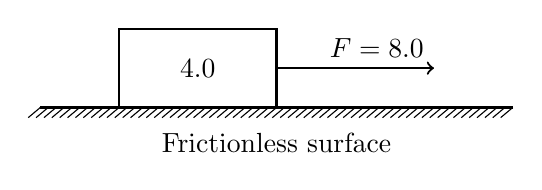
\begin{tikzpicture}
        %% Block
        \draw[thick] (-2,0) rectangle (0,1);
        \node[anchor=center] at (-1.0,0.5) {\SI{4.0}{\kilo\gram}};
        %% Force 1
        \draw[thick,->] (0,0.5) -- (2.00,0.5)
            node[pos=1.0,anchor=south east] {$F=\SI{8.0}{\newton}$};
        %% Floor
        \draw[thick] (-3,0) -- (3,0);
        \foreach \x in {-30,-29,...,30}
            \draw[thin] (\x mm,0cm) -- ++ (220:0.20cm);
        \node[anchor=north] at (0,-0.20) {Frictionless surface};
    \end{tikzpicture}
    \end{center}
    What is the magnitude of the block's acceleration?
    \begin{multicols}{2}
    \begin{choices}
        \wrongchoice{\SI{0.50}{\meter\per\second\squared}}
      \correctchoice{\SI{2.0}{\meter\per\second\squared}}
        \wrongchoice{\SI{9.8}{\meter\per\second\squared}}
        \wrongchoice{\SI{32}{\meter\per\second\squared}}
    \end{choices}
    \end{multicols}
\end{question}
}

\newcommand{\nysedJuneTwentyZeroTwoQTwelve}{
\begin{tikzpicture}
    %% Ground
    \node[anchor=north,fill,pattern=north east lines,minimum width=8cm, minimum height=0.05cm] at (0,0) {};
    \draw (-4,0) -- (4,0);
    %% carts
    \node[draw,minimum width=2cm,minimum height=2em,anchor=south] (A) at (-2,0.3) {\SI{2}{\kilo\gram}};
    \node[draw,minimum width=1cm,minimum height=2em,anchor=south] (B) at (2,0.3) {\SI{1}{\kilo\gram}};
    \node[anchor=south] at (A.north) {$A$};
    \node[anchor=south] at (B.north) {$B$};
    %% wheels
    \draw[fill=white!90!black] (A.south west) ++(0:0.2cm) arc(90:-270:0.15);
    \draw[fill=white!90!black] (A.south east) ++(180:0.2cm) arc(90:-270:0.15);
    \draw[fill=white!90!black] (B.south west) ++(0:0.2cm) arc(90:-270:0.15);
    \draw[fill=white!90!black] (B.south east) ++(180:0.2cm) arc(90:-270:0.15);
    %% Spring
    \draw[decoration={aspect=0.2,segment length=1.5mm,amplitude=2mm,coil},decorate] (A.east) -- (B.west);
    \draw[thick] (A.north east) -- (B.north west);
\end{tikzpicture}
}

\element{nysed}{
\begin{question}{June2002-Q12}
    The diagram shows a compressed spring between two carts initially at rest on a horizontal frictionless surface.
    Cart $A$ has a mass of 2 kilograms and cart $B$ has a mass of \SI{1}{\kilo\gram}.
    A string holds the carts together.
    \begin{center}
        \nysedJuneTwentyZeroTwoQTwelve
    \end{center}
    What occurs when the string is cut and the carts move apart?
    \begin{choices}
      \correctchoice{The magnitude of the acceleration of cart $A$ is one-half the magnitude of the acceleration of cart $B$.}
        \wrongchoice{The length of time that the force acts on cart $A$ is twice the length of time the force acts on cart $B$.}
        \wrongchoice{The magnitude of the force exerted on cart $A$ is one-half the magnitude of the force exerted on cart $B$.}
        \wrongchoice{The magnitude of the impulse applied to cart $A$ is twice the magnitude of the impulse applied to cart $B$.}
    \end{choices}
\end{question}
}

\element{nysed}{
\begin{question}{June2002-Q13}
    The diagram shows a compressed spring between two carts initially at rest on a horizontal frictionless surface.
    Cart $A$ has a mass of 2 kilograms and cart $B$ has a mass of \SI{1}{\kilo\gram}.
    A string holds the carts together.
    \begin{center}
        \nysedJuneTwentyZeroTwoQTwelve
    \end{center}
    After the string is cut and the two carts move apart,
        the magnitude of which quantity is the same for both carts?
    \begin{multicols}{2}
    \begin{choices}
      \correctchoice{momentum}
        \wrongchoice{inertia}
        \wrongchoice{velocity}
        \wrongchoice{kinetic energy}
    \end{choices}
    \end{multicols}
\end{question}
}


%% Section Jan2002
%%--------------------
\element{nysed}{
\begin{question}{Jan2002-Q07}
    A \SI{4.0}{\kilo\gram} rock and a \SI{1.0}{\kilo\gram} stone fall freely from rest from a height of \SI{100}{\meter}.
    After they fall for \SI{2.0}{\second},
        the ratio of the rock's speed to the stone's speed is:
    \begin{multicols}{2}
    \begin{choices}
      \correctchoice{$1:1$}
        \wrongchoice{$1:2$}
        \wrongchoice{$2:1$}
        \wrongchoice{$4:1$}
    \end{choices}
    \end{multicols}
\end{question}
}

\element{nysed}{
\begin{question}{Jan2002-Q09}
    In the diagram below,
        a box is on a frictionless horizontal surface with forces $F_1$ and $F_2$ acting as shown.
    \begin{center}
    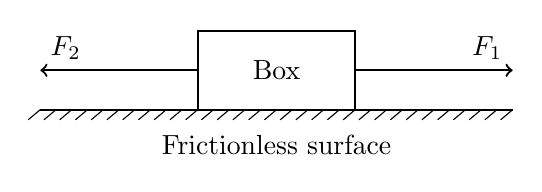
\begin{tikzpicture}
        %% Block
        \draw[thick] (-1,0) rectangle (1,1);
        \node[anchor=center] at (0,0.5) {Box};
        %% Force 1
        \draw[thick,->] (1,0.5) -- (3.00,0.5)
            node[pos=1.0,anchor=south east] {$F_1$};
        %% Force 2
        \draw[thick,->] (-1,0.5) -- (-3.00,0.5)
            node[pos=1.0,anchor=south west] {$F_2$};
        %% Floor
        \draw[thick] (-3,0) -- (3,0);
        \foreach \x in {-30,-28,...,30}
            \draw[thin] (\x mm,0cm) -- ++ (220:0.20cm);
        \node[anchor=north] at (0,-0.20) {Frictionless surface};
    \end{tikzpicture}
    \end{center}
    If the magnitude of $F_1$ is greater than the magnitude of $F_2$,
        then the box is:
    \begin{choices}
        \wrongchoice{moving at constant speed in the direction of $F_1$}
        \wrongchoice{moving at constant speed in the direction of $F_2$}
      \correctchoice{accelerating in the direction of $F_1$}
        \wrongchoice{accelerating in the direction of $F_2$}
    \end{choices}
\end{question}
}

\element{nysed}{
\begin{question}{Jan2002-Q11}
    Which pair of displacement ($d$) and velocity ($v$) graphs best represent the motion of an object on which the net force is zero?
    \begin{choices}
        \AMCboxDimensions{down=-2.5em}
        \correctchoice{
            \begin{tikzpicture}
                \begin{groupplot}[
                    axis lines=middle,
                    axis line style={->},
                    group style={group size=2 by 1},
                    xtick=\empty,
                    x label style={
                        at={(current axis.right of origin)},
                        anchor=west,
                        font=\normalsize,
                    },
                    xmin=0,xmax=10,
                    ytick=\empty,
                    y label style={
                        at={(current axis.above origin)},
                        anchor=south,
                        font=\normalsize,
                    },
                    ymin=0,ymax=10,
                    width=0.5\columnwidth,
                    ]
                    \nextgroupplot[
                        xlabel={$t$},
                        ylabel={$d$},
                    ] \addplot[line width=1pt,domain=0:10] {x};
                    \nextgroupplot[
                        xlabel={$t$},
                        ylabel={$v$},
                    ] \addplot[line width=1pt,domain=0:10] {8};
                \end{groupplot}
            \end{tikzpicture}
        }
        \wrongchoice{
            \begin{tikzpicture}
                \begin{groupplot}[
                    axis lines=middle,
                    axis line style={->},
                    group style={group size=2 by 1},
                    xtick=\empty,
                    x label style={
                        at={(current axis.right of origin)},
                        anchor=west,
                        font=\normalsize,
                    },
                    xmin=0,xmax=10,
                    ytick=\empty,
                    y label style={
                        at={(current axis.above origin)},
                        anchor=south,
                        font=\normalsize,
                    },
                    ymin=0,ymax=10,
                    width=0.5\columnwidth,
                    ]
                    \nextgroupplot[
                        xlabel={$t$},
                        ylabel={$d$},
                    ] \addplot[line width=1pt,domain=0:10] {0.1 * x * x};
                    \nextgroupplot[
                        xlabel={$t$},
                        ylabel={$v$},
                    ] \addplot[line width=1pt,domain=0:10] {x};
                \end{groupplot}
            \end{tikzpicture}
        }
        \wrongchoice{
            \begin{tikzpicture}
                \begin{groupplot}[
                    axis lines=middle,
                    axis line style={->},
                    group style={group size=2 by 1},
                    xtick=\empty,
                    x label style={
                        at={(current axis.right of origin)},
                        anchor=west,
                        font=\normalsize,
                    },
                    xmin=0,xmax=10,
                    ytick=\empty,
                    y label style={
                        at={(current axis.above origin)},
                        anchor=south,
                        font=\normalsize,
                    },
                    ymin=0,ymax=10,
                    width=0.5\columnwidth,
                    ]
                    \nextgroupplot[
                        xlabel={$t$},
                        ylabel={$d$},
                    ] \addplot[line width=1pt,domain=0:10] {x};
                    \nextgroupplot[
                        xlabel={$t$},
                        ylabel={$v$},
                    ] \addplot[line width=1pt,domain=0:10] {0.5*x};
                \end{groupplot}
            \end{tikzpicture}
        }
        \wrongchoice{
            \begin{tikzpicture}
                \begin{groupplot}[
                    axis lines=middle,
                    axis line style={->},
                    group style={group size=2 by 1},
                    xtick=\empty,
                    x label style={
                        at={(current axis.right of origin)},
                        anchor=west,
                        font=\normalsize,
                    },
                    xmin=0,xmax=10,
                    ytick=\empty,
                    y label style={
                        at={(current axis.above origin)},
                        anchor=south,
                        font=\normalsize,
                    },
                    ymin=0,ymax=10,
                    width=0.5\columnwidth,
                    ]
                    \nextgroupplot[
                        xlabel={$t$},
                        ylabel={$d$},
                    ] \addplot[line width=1pt,domain=0:10] {0.1 * x * x};
                    \nextgroupplot[
                        xlabel={$t$},
                        ylabel={$v$},
                    ] \addplot[line width=1pt,domain=0:10] {8};
                \end{groupplot}
            \end{tikzpicture}
        }
    \end{choices}
\end{question}
}

\element{nysed}{
\begin{question}{Jan2002-Q13}
    The magnitude of the force that a baseball bat exerts on a ball is \SI{50}{\newton}.
    The magnitude of the force that the ball exerts on the bat is:
    \begin{multicols}{2}
    \begin{choices}
        \wrongchoice{\SI{5.0}{\newton}}
        \wrongchoice{\SI{10}{\newton}}
      \correctchoice{\SI{50}{\newton}}
        \wrongchoice{\SI{250}{\newton}}
    \end{choices}
    \end{multicols}
\end{question}
}

\element{nysed}{
\begin{question}{Jan2002-Q16}
    What is an essential characteristic of an object in equilibrium?
    \begin{choices}
        \wrongchoice{zero velocity}
      \correctchoice{zero acceleration}
        \wrongchoice{zero potential energy}
        \wrongchoice{zero kinetic energy}
    \end{choices}
\end{question}
}


%% Section June2001
%%--------------------
\element{nysed}{
\begin{question}{June2001-Q07}
    In an automobile collision, a \SI{44}{\kilo\gram} passenger moving at \SI{15}{\meter\per\second} is brought to rest by an air bag during a \SI{0.10}{\second} time interval.
    What is the magnitude of the average force exerted on the passenger during this time?
    \begin{multicols}{2}
    \begin{choices}
        \wrongchoice{\SI{440}{\newton}}
        \wrongchoice{\SI{660}{\newton}}
        \wrongchoice{\SI{4400}{\newton}}
      \correctchoice{\SI{6600}{\newton}}
    \end{choices}
    \end{multicols}
\end{question}
}

\element{nysed}{
\begin{question}{June2001-Q08}
    A series of unbalanced forces was applied to each of two blocks, $A$ and $B$.
    The graphs below show the relationship between unbalanced force and acceleration for each block.
    \begin{center}
    \begin{tikzpicture}
        \begin{groupplot}[
            axis y line=left,
            axis x line=bottom,
            axis line style={->},
            group style={group size=2 by 1},
            xtick={0,1,2,3,4},
            xlabel={acceleration},
            x unit=\si{\meter\per\second\squared},
            xmin=0,xmax=4.5,
            ytick={0,1,2,3},
            ylabel={force},
            y unit=\si{\newton},
            ymin=0,ymax=3.5,
            width=0.5\columnwidth,
            ]
            \nextgroupplot[title={Block $A$}]
            \addplot[line width=1pt,domain=0:3.5] {x};
            \addplot[mark=*] coordinates {(1,1) (2,2) (3,3)};
            \nextgroupplot[title={Block $B$}]
            \addplot[line width=1pt,domain=0:2] {2*x};
            \addplot[mark=*] coordinates {(0.5,1) (1,2) (1.5,3)};
        \end{groupplot}
    \end{tikzpicture}
    \end{center}
    Compared to the mass of block $A$,
        the mass of block $B$ is:
    \begin{multicols}{2}
    \begin{choices}
        \wrongchoice{the same}
      \correctchoice{twice as great}
        \wrongchoice{half as great}
        \wrongchoice{four times as great}
    \end{choices}
    \end{multicols}
\end{question}
}

\element{nysed}{
\begin{question}{June2001-Q55}
    A mosquito flying over a highway strikes the windshield of a moving truck.
    Compared to the magnitude of the force of the truck on the mosquito during the collision,
        the magnitude of the force of the mosquito on the truck is:
    \begin{multicols}{3}
    \begin{choices}
        \wrongchoice{smaller}
        \wrongchoice{larger}
      \correctchoice{the same}
    \end{choices}
    \end{multicols}
\end{question}
}


%% Section Jan2001
%%--------------------
\element{nysed}{
\begin{question}{Jan2001-Q08}
    Which is a derived unit?
    \begin{multicols}{2}
    \begin{choices}
        \wrongchoice{meter (\si{\meter})}
        \wrongchoice{kilogram (\si{\kilo\gram})}
        \wrongchoice{second (\si{\kilo\gram})}
      \correctchoice{newton (\si{\newton})}
    \end{choices}
    \end{multicols}
\end{question}
}

\element{nysed}{
\begin{question}{Jan2001-Q13}
    A \SI{2.0}{\kilo\gram} mass weights \SI{10}{\newton} on planet $X$.
    The acceleration due to gravity on planet $X$ is approximately:
    \begin{multicols}{2}
    \begin{choices}
        \wrongchoice{\SI{0.20}{\meter\per\second\squared}}
      \correctchoice{\SI{5.0}{\meter\per\second\squared}}
        \wrongchoice{\SI{9.8}{\meter\per\second\squared}}
        \wrongchoice{\SI{20}{\meter\per\second\squared}}
    \end{choices}
    \end{multicols}
\end{question}
}


%% Section June2000
%%--------------------
\element{nysed}{
\begin{question}{June2000-Q12}
    Two forces are applied to a \SI{2.0}{\kilo\gram} block on a frictionless horizontal surface,
        as shown in the diagram below.
    [Vectors are drawn to scale]
    \begin{center}
    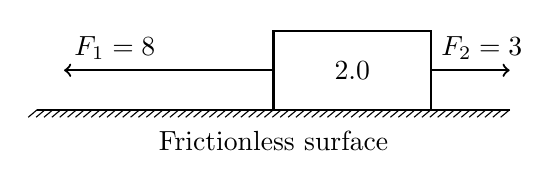
\begin{tikzpicture}
        %% Force 1
        \draw[thick,->] (-0,0.5) -- (-2.66,0.5)
            node[pos=1.0,anchor=south west] {$F_1=\SI{8}{\newton}$};
        %% Force 2
        \draw[thick,->] (2,0.5) -- (3.00,0.5)
            node[pos=0.0,anchor=south west] {$F_2=\SI{3}{\newton}$};
        %% Block
        \draw[thick] (0,0) rectangle (2,1);
        \node[anchor=center] at (1,0.5) {\SI{2.0}{\kilo\gram}};
        %% Floor
        \draw[thick] (-3,0) -- (3,0);
        \foreach \x in {-30,-29,...,30}
            \draw[thin] (\x mm,0cm) -- ++ (220:0.15cm);
        \node[anchor=north] at (0,-0.15) {Frictionless surface};
    \end{tikzpicture}
    \end{center}
    The acceleration of the block is:
    \begin{choices}
        \wrongchoice{\SI{1.5}{\meter\per\second\squared} to the right}
      \correctchoice{\SI{2.5}{\meter\per\second\squared} to the left}
        \wrongchoice{\SI{2.5}{\meter\per\second\squared} to the right}
        \wrongchoice{\SI{4.0}{\meter\per\second\squared} to the left}
    \end{choices}
\end{question}
}

\element{nysed}{
\begin{question}{June2000-Q13}
    A \SI{15}{\kilo\gram} mass weighs \SI{60}{\newton} on planet $X$.
    The mass is allowed to fall freely from rest near the surface of the planet.
    After falling for \SI{6.0}{\second},
        the acceleration of the mass is:
    \begin{multicols}{2}
    \begin{choices}
        \wrongchoice{\SI{0.25}{\meter\per\second\squared}}
        \wrongchoice{\SI{10}{\meter\per\second\squared}}
        \wrongchoice{\SI{24}{\meter\per\second\squared}}
      \correctchoice{\SI{4.0}{\meter\per\second\squared}}
    \end{choices}
    \end{multicols}
\end{question}
}

\element{nysed}{
\begin{question}{June2000-Q17}
    A \SI{2 400}{\kilo\gram} car is traveling at a speed of \SI{20}{\meter\per\second}.
    Compared to the magnitude of the force required to stop the car in \SI{12}{\second},
        the magnitude of the force required to stop the car in \SI{6}{\second} is:
    \begin{choices}
        \wrongchoice{half as great}
      \correctchoice{twice as great}
        \wrongchoice{the same}
        \wrongchoice{four times as great}
    \end{choices}
\end{question}
}


%% Section June1999
%%--------------------
\element{nysed}{
\begin{question}{June1999-Q04}
    A \SI{1.2e3}{\kilo\gram} car is accelerated uniformly from \SI{10}{\meter\per\second} to \SI{20}{\meter\per\second} in \SI{5.0}{\second}.
    What is the magnitude of the net force acting on the car during this \SI{5.0}{\second} interval?
    \begin{multicols}{2}
    \begin{choices}
      \correctchoice{\SI{2.4e3}{\newton}}
        \wrongchoice{\SI{4.8e3}{\newton}}
        \wrongchoice{\SI{7.2e3}{\newton}}
        \wrongchoice{\SI{1.2e4}{\newton}}
    \end{choices}
    \end{multicols}
\end{question}
}

\element{nysed}{
\begin{question}{June1999-Q09}
    The diagram below shows a student applying a \SI{10}{\newton} force to slide a piece of wood at constant speed across a horizontal surface.
    After the wood is cut in half,
        one piece is placed on top of the other, as shown.
    \begin{center}
    \begin{tikzpicture}
        %% NOTE: add picture
    \end{tikzpicture}
    \end{center}
    What is the magnitude of the force, $F$,
        required to slide the stacked wood at constant speed across the surface?
    \begin{multicols}{2}
    \begin{choices}
        \wrongchoice{\SI{40}{\newton}}
        \wrongchoice{\SI{20}{\newton}}
      \correctchoice{\SI{10}{\newton}}
        \wrongchoice{\SI{5.0}{\newton}}
    \end{choices}
    \end{multicols}
\end{question}
}

\element{nysed}{
\begin{question}{June1999-Q11}
    Which combination of fundamental units can be used to express the weight of an object?
    \begin{choices}
        \wrongchoice{kilogram per second (\si{\kilo\gram\per\second})}
        \wrongchoice{kilogram meter (\si{\kilo\gram\meter})}
        \wrongchoice{kilogram meter per second (\si{\kilo\gram\meter\per\second})}
      \correctchoice{kilogram meter per second squared (\si{\kilo\gram\meter\per\second\squared})}
    \end{choices}
\end{question}
}

\element{nysed}{
\begin{question}{June1999-Q15}
    The diagram below shows a child pulling a \SI{50}{\kilo\gram} friend on a sled by applying a \SI{300}{\newton} force on the sled rope at an angle of \ang{40} with the horizontal.
    \begin{center}
        %% NOTE: too complex for tikz
        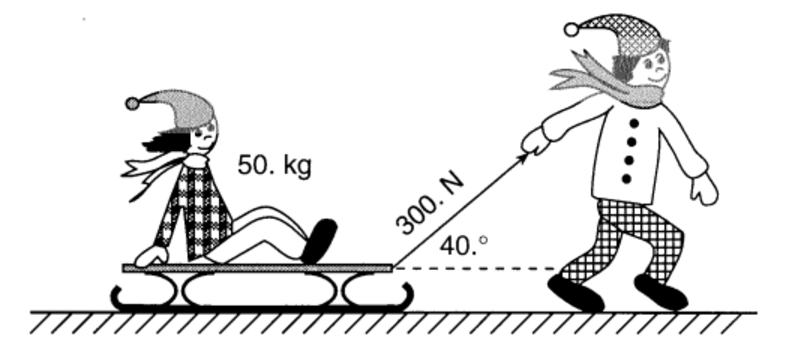
\includegraphics[keepaspectratio,scale=0.5]{June1999-Q15}
    \end{center}
    The vertical component of the \SI{300}{\newton} force is approximately:
    \begin{multicols}{2}
    \begin{choices}
        \wrongchoice{\SI{510}{\newton}}
        \wrongchoice{\SI{230}{\newton}}
      \correctchoice{\SI{190}{\newton}}
        \wrongchoice{\SI{32}{\newton}}
    \end{choices}
    \end{multicols}
\end{question}
}

\element{nysed}{
\begin{question}{June1999-Q17}
    A \SI{6.0}{\newton} force and a \SI{8}{\newton} force act concurrently on a box located on a frictionless horizontal surface.
    Which top-view diagram shows the forces producing the \emph{smallest} magnitude of acceleration of the box?
    \begin{multicols}{2}
    \begin{choices}[o]
        \footnotesize
        \AMCboxDimensions{down=-1.1cm}
        \correctchoice{
            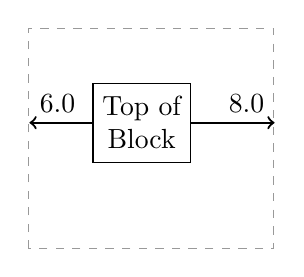
\begin{tikzpicture}[scale=0.8]
                \draw[white!60!black,dashed] (-1.8,-2.0) rectangle (2.10,1.5);
                %% Block
                \node[draw,rectangle,minimum size=1cm,text centered,text width=1cm]
                    (B) at (0,0) {Top of Block};
                %% 8 Newton
                \draw[thick,->] (B.east) -- ++(0:1.33cm)
                    node[pos=1.0,anchor=south east] {\SI{8.0}{\newton}};
                %% 6 Newton
                \draw[thick,->] (B.west) -- ++(180:1.00cm)
                    node[pos=1.0,anchor=south west] {\SI{6.0}{\newton}};
            \end{tikzpicture}
        }
        \wrongchoice{
            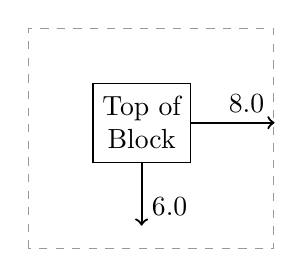
\begin{tikzpicture}[scale=0.8]
                \draw[white!60!black,dashed] (-1.8,-2.0) rectangle (2.10,1.5);
                %% Block
                \node[draw,rectangle,minimum size=1cm,text centered,text width=1cm]
                    (B) at (0,0) {Top of Block};
                %% 8 Newton
                \draw[thick,->] (B.east) -- ++(0:1.33cm)
                    node[pos=1.0,anchor=south east] {\SI{8.0}{\newton}};
                %% 6 Newton
                \draw[thick,->] (B.south) -- ++(270:1.00cm)
                    node[pos=1.0,anchor=south west] {\SI{6.0}{\newton}};
            \end{tikzpicture}
        }
        \wrongchoice{
            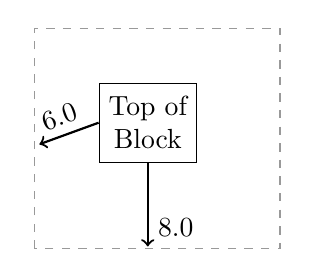
\begin{tikzpicture}[scale=0.8]
                \draw[white!60!black,dashed] (-1.8,-2.0) rectangle (2.10,1.5);
                %% Block
                \node[draw,rectangle,minimum size=1cm,text centered,text width=1cm]
                    (B) at (0,0) {Top of Block};
                %% 8 Newton
                \draw[thick,->] (B.south) -- ++(270:1.33cm)
                    node[pos=1.0,anchor=south west] {\SI{8.0}{\newton}};
                %% 6 Newton
                \draw[thick,->] (B.west) -- ++(200:1.00cm)
                    node[pos=1.0,anchor=south west,rotate=20] {\SI{6.0}{\newton}};
            \end{tikzpicture}
        }
        \wrongchoice{
            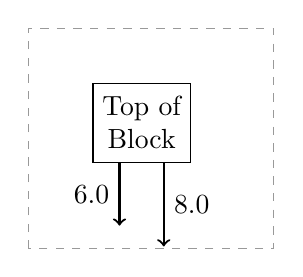
\begin{tikzpicture}[scale=0.8]
                \draw[white!60!black,dashed] (-1.8,-2.0) rectangle (2.10,1.5);
                %% Block
                \node[draw,rectangle,minimum size=1cm,text centered,text width=1cm]
                    (B) at (0,0) {Top of Block};
                %% 8 Newton
                \draw[thick,->] (B.south)++(10pt,0) -- ++(270:1.33cm)
                    node[pos=0.5,anchor=west] {\SI{8.0}{\newton}};
                %% 6 Newton
                \draw[thick,->] (B.south)++(-10pt,0) -- ++(270:1.00cm)
                    node[pos=0.5,anchor=east] {\SI{6.0}{\newton}};
            \end{tikzpicture}
        }
    \end{choices}
    \end{multicols}
\end{question}
}


%% Section June1998
%%--------------------
\element{nysed}{
\begin{question}{June1998-Q08}
    A man weighs \SI{900}{\newton} standing on a scale in a stationary elevator.
    If some time later the reading on the scale is \SI{1200}{\newton},
        the elevator must be moving with:
    \begin{choices}
        \wrongchoice{constant acceleration downward}
        \wrongchoice{constant speed downward}
      \correctchoice{constant acceleration upward}
        \wrongchoice{constant speed upward}
    \end{choices}
\end{question}
}

\element{nysed}{
\begin{question}{June1998-Q09}
    Net force $F$ causes $m_1$ to accelerate at rate $a$.
    A net force of $3F$ causes mass $m_2$ to accelerate at rate $2a$.
    What is the ratio of mass $m_1$ to mass $m_2$?
    \begin{multicols}{2}
    \begin{choices}
        \wrongchoice{$1:3$}
      \correctchoice{$2:3$}
        \wrongchoice{$1:2$}
        \wrongchoice{$1:6$}
    \end{choices}
    \end{multicols}
\end{question}
}

\element{nysed}{
\begin{question}{June1998-Q13}
    A \SI{0.60}{\kilo\gram} softball initially at rest is hit with a bat.
    The ball is in contact with the bat for \SI{0.20}{\second} and leaves the bat with a speed of \SI{25}{\meter\per\second}.
    What is the magnitude of the average force exerted by the ball on the bat?
    \begin{multicols}{2}
    \begin{choices}
        \wrongchoice{\SI{8.3}{\newton}}
        \wrongchoice{\SI{15}{\newton}}
        \wrongchoice{\SI{3.0}{\newton}}
      \correctchoice{\SI{75}{\newton}}
    \end{choices}
    \end{multicols}
\end{question}
}

\element{nysed}{
\begin{question}{June1998-Q16}
    A person kicks a \SI{4.0}{\kilo\gram} door with a \SI{48}{\newton} force causing the door to accelerate at \SI{12}{\meter\per\second\squared}.
    What is the magnitude of the force exerted by the door on the person?
    \begin{multicols}{2}
    \begin{choices}
      \correctchoice{\SI{48}{\newton}}
        \wrongchoice{\SI{24}{\newton}}
        \wrongchoice{\SI{12}{\newton}}
        \wrongchoice{\SI{4.0}{\newton}}
    \end{choices}
    \end{multicols}
\end{question}
}


%% Section June1997
%%--------------------
\element{nysed}{
\begin{question}{June1997-Q05}
    A \SI{150}{\newton} force, $F_1$, and a \SI{200}{\newton} force,
        $F_2$, are applied simultaneously to the same point on a large crate resting on a frictionless, horizontal surface.
    Which diagram shows the forces positioned to give the crate the greatest acceleration?
    [Vectors are drawn to scale]
    \begin{multicols}{2}
    \begin{choices}
        \AMCboxDimensions{down=-0.25cm}
        \correctchoice{
            \begin{tikzpicture}[scale=0.75]
                \draw[white] (-2,-0.5) rectangle (2,2.33);
                %% Block
                \node[draw,rectangle,minimum size=0.8cm,anchor=south] (B) at (-0.5,0) {};
                %% F_1
                \draw[thick,->] (B.north east) -- ++(0:1.25)
                    node[pos=1.0,anchor=south east] {$F_1$};
                %% F_2
                \draw[thick,->] (B.east) -- ++(0:1.66)
                    node[pos=1.0,anchor=south] {$F_2$};
                %% Floor
                \draw[thick] (-2,0) -- (2,0);
                \node[anchor=north,pattern=north east lines,minimum width=3cm] at (0,0) {};
            \end{tikzpicture}
        }
        \wrongchoice{
            \begin{tikzpicture}[scale=0.75]
                \draw[white] (-2,-0.5) rectangle (2,2.33);
                %% Block
                \node[draw,rectangle,minimum size=0.8cm,anchor=south] (B) at (-0.5,0) {};
                %% F_1
                \draw[thick,<-] (B.north) -- ++(90:1.25)
                    node[pos=0.0,anchor=south east] {$F_1$};
                %% F_2
                \draw[thick,->] (B.east) -- ++(0:1.66)
                    node[pos=1.0,anchor=south east] {$F_2$};
                %% Floor
                \draw[thick] (-2,0) -- (2,0);
                \node[anchor=north,pattern=north east lines,minimum width=3cm] at (0,0) {};
            \end{tikzpicture}
        }
        \wrongchoice{
            \begin{tikzpicture}[scale=0.75]
                \draw[white] (-2,-0.5) rectangle (2,2.33);
                %% Block
                \node[draw,rectangle,minimum size=0.8cm,anchor=south] (B) at (-0.5,0) {};
                %% F_1
                \draw[thick,->] (B.north) -- ++(90:1.25)
                    node[pos=1.0,anchor=north east] {$F_1$};
                %% F_2
                \draw[thick,->] (B.east) -- ++(0:1.66)
                    node[pos=1.0,anchor=south east] {$F_2$};
                %% Floor
                \draw[thick] (-2,0) -- (2,0);
                \node[anchor=north,pattern=north east lines,minimum width=3cm] at (0,0) {};
            \end{tikzpicture}
        }
        \wrongchoice{
            \begin{tikzpicture}[scale=0.75]
                \draw[white] (-2,-0.5) rectangle (2,2.33);
                %% Block
                \node[draw,rectangle,minimum size=0.8cm,anchor=south] (B) at (-0.5,0) {};
                %% F_1
                \draw[thick,->] (B.west) -- ++(180:1.25)
                    node[pos=1.0,anchor=south west] {$F_1$};
                %% F_2
                \draw[thick,->] (B.east) -- ++(0:1.66)
                    node[pos=1.0,anchor=south east] {$F_2$};
                %% Floor
                \draw[thick] (-2,0) -- (2,0);
                \node[anchor=north,pattern=north east lines,minimum width=3cm] at (0,0) {};
            \end{tikzpicture}
        }
    \end{choices}
    \end{multicols}
\end{question}
}

\element{nysed}{
\begin{question}{June1997-Q11}
    The graph below shows the weight of three objects on planet $X$ as a function of their mass.
    \begin{center}
    \begin{tikzpicture}
        \begin{axis}[
            axis y line=left,
            axis x line=bottom,
            axis line style={->},
            ylabel={Weight},
            y unit=\si{\newton},
            ytick={0,100,200,300,400,500},
            xlabel={Mass},
            x unit=\si{\kilo\gram},
            xtick={0,25,50,75},
            xmin=0,xmax=77,
            ymin=0,ymax=510,
            grid=major,
            width=0.8\columnwidth,
            height=0.5\columnwidth,
            very thin,
        ]
        \addplot[line width=1pt,domain=0:75]{6.0* x};
        \addplot[mark=*] coordinates {(25,150) (50,300) (75,450)};
        \end{axis}
    \end{tikzpicture}
    \end{center}
    The acceleration due to gravity on planet $X$ is approximately:
    \begin{multicols}{2}
    \begin{choices}
        \wrongchoice{\SI{0.17}{\meter\per\second\squared}}
      \correctchoice{\SI{6.0}{\meter\per\second\squared}}
        \wrongchoice{\SI{9.8}{\meter\per\second\squared}}
        \wrongchoice{\SI{50}{\meter\per\second\squared}}
    \end{choices}
    \end{multicols}
\end{question}
}

\element{nysed}{
\begin{question}{June1997-Q12}
    What is the magnitude of the net force acting on a \SI{2.0e3}{\kilo\gram} car as it accelerates from rest to a speed of \SI{15}{\meter\per\second} in \SI{5.0}{\second}?
    \begin{multicols}{2}
    \begin{choices}
      \correctchoice{\SI{6.0e3}{\newton}}
        \wrongchoice{\SI{2.0e4}{\newton}}
        \wrongchoice{\SI{3.0e4}{\newton}}
        \wrongchoice{\SI{6.0e4}{\newton}}
    \end{choices}
    \end{multicols}
\end{question}
}


%% Section June1996
%%--------------------
\element{nysed}{
\begin{question}{June1996-Q07}
    A \SI{0.4}{\kilo\gram} rock and a \SI{1.0}{\kilo\gram} stone fall freely from rest from a height of \SI{100}{\meter}.
    After they fall for \SI{2.0}{\second},
        the ratio of the rock's speed to the stone's speed is:
    \begin{multicols}{2}
    \begin{choices}
      \correctchoice{$1:1$}
        \wrongchoice{$2:1$}
        \wrongchoice{$1:2$}
        \wrongchoice{$4:1$}
    \end{choices}
    \end{multicols}
\end{question}
}

%\element{nysed}{
%\begin{question}{June1996-Q09}
%    The diagram below shows a person exerting a \SI{300}{\newton} force on the handle of a shovel that makes an angle of \ang{60} with the horizontal ground.
%    \begin{center}
%        %% NOTE: picture of a person holding a shovel
%    \end{center}
%    The component of the \SI{300}{\newton} force that acts perpendicular to the ground is approximately:
%    \begin{multicols}{2}
%    \begin{choices}
%        \wrongchoice{\SI{150}{\newton}}
%      \correctchoice{\SI{260}{\newton}}
%        \wrongchoice{\SI{300}{\newton}}
%        \wrongchoice{\SI{350}{\newton}}
%    \end{choices}
%    \end{multicols}
%\end{question}
%}

\element{nysed}{
\begin{question}{June1996-Q10}
    Which graph best represents the motion of an object that has \emph{no} unbalanced force acting on it?
    \begin{multicols}{2}
    \begin{choices}
        \AMCboxDimensions{down=-2.5em}
        \correctchoice{
            \begin{tikzpicture}
                \begin{axis}[
                    axis y line=left,
                    axis x line=bottom,
                    axis line style={->},
                    xlabel={time},
                    xtick=\empty,
                    ylabel={displacement},
                    ytick=\empty,
                    xmin=0,xmax=11,
                    ymin=0,ymax=11,
                    width=1.0\columnwidth,
                ]
                \addplot[line width=1pt,domain=0:10]{0.1*x*x};
                \end{axis}
            \end{tikzpicture}
        }
        \wrongchoice{
            \begin{tikzpicture}
                \begin{axis}[
                    axis y line=left,
                    axis x line=bottom,
                    axis line style={->},
                    xlabel={time},
                    xtick=\empty,
                    ylabel={acceleration},
                    ytick=\empty,
                    xmin=0,xmax=11,
                    ymin=0,ymax=11,
                    width=1.0\columnwidth,
                ]
                \addplot[line width=1pt,domain=0:10]{x};
                \end{axis}
            \end{tikzpicture}
        }
        \wrongchoice{
            \begin{tikzpicture}
                \begin{axis}[
                    axis y line=left,
                    axis x line=bottom,
                    axis line style={->},
                    xlabel={time},
                    xtick=\empty,
                    ylabel={momentum},
                    ytick=\empty,
                    xmin=0,xmax=11,
                    ymin=0,ymax=11,
                    width=1.0\columnwidth,
                ]
                \addplot[line width=1pt,domain=0:10]{x};
                \end{axis}
            \end{tikzpicture}
        }
        \wrongchoice{
            \begin{tikzpicture}
                \begin{axis}[
                    axis y line=left,
                    axis x line=bottom,
                    axis line style={->},
                    xlabel={time},
                    xtick=\empty,
                    ylabel={velocity},
                    ytick=\empty,
                    xmin=0,xmax=11,
                    ymin=0,ymax=11,
                    width=1.0\columnwidth,
                ]
                \addplot[line width=1pt,domain=0:10]{0.1*x*x};
                \end{axis}
            \end{tikzpicture}
        }
    \end{choices}
    \end{multicols}
\end{question}
}

\element{nysed}{
\begin{question}{June1996-Q12}
    Two forces are applied to a \SI{2.0}{\kilo\gram} block on a frictionless,
        horizontal surface, as shown in the diagram below.
    \begin{center}
    \begin{tikzpicture}
        %% Force 1
        \draw[thick,->] (-2.0,0.5) -- (-2.75,0.5)
            node[pos=0.0,anchor=south east] {$F_1=\SI{2}{\newton}$};
        %% Force 2
        \draw[thick,->] (0,0.5) -- (3.0,0.5)
            node[pos=1.0,anchor=south east] at (2,0.5) {$F_2=\SI{8}{\newton}$};
        %% Block
        \draw[thick] (0,0) rectangle (-2,1);
        \node[anchor=center] at (-1,0.5) {\SI{2.0}{\kilo\gram}};
        %% Floor
        \draw[thick] (-3,0) -- (3,0);
        \node[anchor=north,minimum width=6cm,pattern=north east lines] at (0,0) {};
        \node[anchor=north,yshift=-1em] at (0,0) {Frictionless surface};
    \end{tikzpicture}
    \end{center}
    The acceleration of the block is:
    \begin{choices}
        \wrongchoice{\SI{5.0}{\meter\per\second\squared} to the right}
        \wrongchoice{\SI{5.0}{\meter\per\second\squared} to the left}
      \correctchoice{\SI{3.0}{\meter\per\second\squared} to the right}
        \wrongchoice{\SI{3.0}{\meter\per\second\squared} to the left}
    \end{choices}
\end{question}
}

\element{nysed}{
\begin{question}{June1996-Q13}
    Compared to the inertia of a \SI{0.10}{\kilo\gram} steel ball,
        the inertia of a \SI{0.20}{\kilo\gram} styrofoam ball is:
    \begin{multicols}{2}
    \begin{choices}
        \wrongchoice{one-half as great}
      \correctchoice{twice as great}
        \wrongchoice{the same}
        \wrongchoice{four times as great}
    \end{choices}
    \end{multicols}
\end{question}
}

\element{nysed}{
\begin{question}{June1996-Q15}
    As shown in the diagram below,
        an inflated balloon released from rest move horizontally with velocity $v$.
    \begin{center}
    \begin{tikzpicture}
        %% balloon
        \draw (0,1ex) to[out=0,in=180] (2,1) arc (90:-90:1) to[out=180,in=0] (0,-1ex);
        \draw[thick] (0,0) circle (0.25ex and 1ex);
        \node[anchor=center] at (2,0) {Balloon};
        \draw[thick,->] (1.5,1.25) -- ++(0:1) node[pos=0.5,anchor=south] {$v$};
        %% Air
        \foreach \x in {1,2,...,50} \fill ({-0.5 - 1*rnd},{0.25*rand}) circle (0.5pt);
        \node[anchor=south] at (-1,0.5) {air};
        \draw[thick,->] (-0.25,0) -- (180:2);
    \end{tikzpicture}
    \end{center}
    The velocity of the balloon is most likely cause by:
    \begin{choices}
      \correctchoice{action-reaction}
        \wrongchoice{centripetal force}
        \wrongchoice{gravitational attraction}
        \wrongchoice{rolling friction}
    \end{choices}
\end{question}
}


%% Section June1995
%%--------------------
\element{nysed}{
\begin{question}{June1995-Q07}
    Which combination of concurrent forces could \emph{not} produce equilibrium?
    \begin{choices}
      \correctchoice{\SI{10}{\newton}, \SI{20}{\newton}, and \SI{50}{\newton}}
        \wrongchoice{\SI{20}{\newton}, \SI{30}{\newton}, and \SI{50}{\newton}}
        \wrongchoice{\SI{30}{\newton}, \SI{40}{\newton}, and \SI{50}{\newton}}
        \wrongchoice{\SI{40}{\newton}, \SI{40}{\newton}, and \SI{50}{\newton}}
    \end{choices}
\end{question}
}

\element{nysed}{
\begin{question}{June1995-Q08}
    A \SI{60}{\kilo\gram} astronaut weighs \SI{96}{\newton} on the surface of the Moon.
    The acceleration due to gravity on the Moon is:
    \begin{multicols}{2}
    \begin{choices}
        \wrongchoice{\SI{0.0}{\meter\per\second\squared}}
      \correctchoice{\SI{1.6}{\meter\per\second\squared}}
        \wrongchoice{\SI{4.9}{\meter\per\second\squared}}
        \wrongchoice{\SI{9.8}{\meter\per\second\squared}}
    \end{choices}
    \end{multicols}
\end{question}
}

\element{nysed}{
\begin{question}{June1995-Q11}
    A student weighing \SI{500}{\newton} stands on a spring scale in an elevator.
    If the scale reads \SI{520}{\newton}, the elevator must be:
    \begin{choices}
      \correctchoice{accelerating upward}
        \wrongchoice{accelerating downward}
        \wrongchoice{moving upward at constant speed}
        \wrongchoice{moving downward at constant speed}
    \end{choices}
\end{question}
}

\element{nysed}{
\begin{question}{June1995-Q52}
    As the angle between a force and level ground decreases from \ang{60} to \ang{30},
        the vertical component of the force:
    \begin{choices}
      \correctchoice{decreases}
        \wrongchoice{increases}
        \wrongchoice{remains the same}
    \end{choices}
\end{question}
}

\element{nysed}{
\begin{question}{June1995-Q53}
    In a baseball game,
        a batter hits a ball for a home run.
    Compared to the magnitude of the impulse imparted to the ball,
        the magnitude of the impulse imparted to the bat is:
    \begin{multicols}{3}
    \begin{choices}
        \wrongchoice{less}
        \wrongchoice{greater}
      \correctchoice{the same}
    \end{choices}
    \end{multicols}
\end{question}
}


%% Section June1994
%%--------------------
\element{nysed}{
\begin{question}{June1994-Q02}
    Which two graphs represent the motion of an object on which the net force is zero?
    \begin{choices}
        \AMCboxDimensions{down=-2.5em}
        \wrongchoice{
            \begin{tikzpicture}
                \begin{groupplot}[
                        axis y line=left,
                        axis x line=bottom,
                        axis line style={->},
                        group style={group size=2 by 1},
                        xtick=\empty,
                        ytick=\empty,
                        width=0.5\columnwidth,
                    ]
                    \nextgroupplot[
                        xlabel={time},
                        ylabel={distance},
                        xmin=0,xmax=11,
                        ymin=0,ymax=11,
                    ] \addplot[line width=1pt,domain=0:10] {x};
                    \nextgroupplot[
                        xlabel={time},
                        ylabel={speed},
                        xmin=0,xmax=11,
                        ymin=0,ymax=11,
                    ] \addplot[line width=1pt,domain=0:10] {0.5*x};
                \end{groupplot}
            \end{tikzpicture}
        }
        %% ANS is 2
        \correctchoice{
            \begin{tikzpicture}
                \begin{groupplot}[
                        axis y line=left,
                        axis x line=bottom,
                        axis line style={->},
                        group style={group size=2 by 1},
                        xtick=\empty,
                        ytick=\empty,
                        width=0.5\columnwidth,
                    ]
                    \nextgroupplot[
                        xlabel={time},
                        ylabel={distance},
                        xmin=0,xmax=11,
                        ymin=0,ymax=11,
                    ] \addplot[line width=1pt,domain=0:10] {x};
                    \nextgroupplot[
                        xlabel={time},
                        ylabel={speed},
                        xmin=0,xmax=11,
                        ymin=0,ymax=11,
                    ] \addplot[line width=1pt,domain=0:10] {7};
                \end{groupplot}
            \end{tikzpicture}
        }
        \wrongchoice{
            \begin{tikzpicture}
                \begin{groupplot}[
                        axis y line=left,
                        axis x line=bottom,
                        axis line style={->},
                        group style={group size=2 by 1},
                        xtick=\empty,
                        ytick=\empty,
                        width=0.5\columnwidth,
                    ]
                    \nextgroupplot[
                        xlabel={time},
                        ylabel={distance},
                        xmin=0,xmax=11,
                        ymin=0,ymax=11,
                    ] \addplot[line width=1pt,domain=0:10] {0.1*x*x};
                    \nextgroupplot[
                        xlabel={time},
                        ylabel={speed},
                        xmin=0,xmax=11,
                        ymin=0,ymax=11,
                    ] \addplot[line width=1pt,domain=0:10] {0.5*x};
                \end{groupplot}
            \end{tikzpicture}
        }
        \wrongchoice{
            \begin{tikzpicture}
                \begin{groupplot}[
                        axis y line=left,
                        axis x line=bottom,
                        axis line style={->},
                        group style={group size=2 by 1},
                        xtick=\empty,
                        ytick=\empty,
                        width=0.5\columnwidth,
                    ]
                    \nextgroupplot[
                        xlabel={time},
                        ylabel={distance},
                        xmin=0,xmax=11,
                        ymin=0,ymax=11,
                    ] \addplot[line width=1pt,domain=0:10] {0.1*x*x};
                    \nextgroupplot[
                        xlabel={time},
                        ylabel={speed},
                        xmin=0,xmax=11,
                        ymin=0,ymax=11,
                    ] \addplot[line width=1pt,domain=0:10] {7};
                \end{groupplot}
            \end{tikzpicture}
        }
    \end{choices}
\end{question}
}

\element{nysed}{
\begin{question}{June1994-Q12}
    A net force of \SI{5.0e2}{\newton} causes an object to accelerated at a rate of \SI{5.0}{\meter\per\second\squared}.
    What is the mass of the object?
    \begin{multicols}{2}
    \begin{choices}
      \correctchoice{\SI{1.0e2}{\kilo\gram}}
        \wrongchoice{\SI{2.0e-1}{\kilo\gram}}
        \wrongchoice{\SI{6.0e2}{\kilo\gram}}
        \wrongchoice{\SI{2.5e3}{\kilo\gram}}
    \end{choices}
    \end{multicols}
\end{question}
}

\element{nysed}{
\begin{question}{June1994-Q14}
    The mass of a space shuttle is approximately \SI{2.0e6}{\kilo\gram}.
    During lift-off, the net force on the shuttle is \SI{1.0e7}{\newton} directed upward.
    What is the speed of the shuttle \SI{10}{\second} after lift-off?
    [Neglect air resistance and the mass change of the shuttle.]
    \begin{multicols}{2}
    \begin{choices}
        \wrongchoice{\SI{5.0e0}{\meter\per\second}}
      \correctchoice{\SI{5.0e1}{\meter\per\second}}
        \wrongchoice{\SI{5.0e2}{\meter\per\second}}
        \wrongchoice{\SI{5.0e3}{\meter\per\second}}
    \end{choices}
    \end{multicols}
\end{question}
}


%% Section June1990
%%--------------------
\element{nysed}{
\begin{question}{June1990-Q08}
    A force of \SI{6.0}{\newton} north and a force of \SI{8.0}{\newton} east act concurrently on an object.
    The magnitude of the resultant of the two forces is:
    \begin{multicols}{2}
    \begin{choices}
        \wrongchoice{\SI{1.3}{\newton}}
        \wrongchoice{\SI{2.0}{\newton}}
      \correctchoice{\SI{10}{\newton}}
        \wrongchoice{\SI{14}{\newton}}
    \end{choices}
    \end{multicols}
\end{question}
}

\element{nysed}{
\begin{question}{June1990-Q10}
    A \SI{50.0}{\kilo\gram} object in outer space is attracted to a nearby planet with a net force of \SI{400}{\newton}.
    What is the magnitude of the object's acceleration?
    \begin{multicols}{2}
    \begin{choices}
      \correctchoice{\SI{8.00}{\meter\per\second\squared}}
        \wrongchoice{\SI{9.81}{\meter\per\second\squared}}
        \wrongchoice{\SI{78.4}{\meter\per\second\squared}}
        \wrongchoice{\SI{2 000}{\meter\per\second\squared}}
    \end{choices}
    \end{multicols}
\end{question}
}


%% Section June1989
%%--------------------
\element{nysed}{
\begin{question}{June1989-Q05}
    The diagram below shows a graph of distance as a function of time for an object in straight-line motion.
    \begin{center}
    \begin{tikzpicture}
        \begin{axis}[
            axis y line=left,
            axis x line=bottom,
            axis line style={->},
            xlabel={time},
            xtick=\empty,
            ylabel={distance},
            ytick=\empty,
            xmin=0,xmax=11,
            ymin=0,ymax=11,
            width=0.8\columnwidth,
            height=0.5\columnwidth,
            very thin,
        ]
        \addplot[line width=1pt,domain=0:10] {0.1*x*x};
        \end{axis}
    \end{tikzpicture}
    \end{center}
    According to the graph, the object most likely has:
    \begin{choices}
        \wrongchoice{constant momentum}
        \wrongchoice{constant acceleration}
        \wrongchoice{a decreasing mass}
      \correctchoice{an increasing speed}
    \end{choices}
\end{question}
}

\element{nysed}{
\begin{question}{June1989-Q09}
    An unbalanced \SI{6.0}{\newton} force acts eastward on an object for \SI{3.0}{\second}.
    The impulse produced by the force is:
    \begin{multicols}{2}
    \begin{choices}
      \correctchoice{\SI{18}{\newton\second} east}
        \wrongchoice{\SI{2.0}{\newton\second} east}
        \wrongchoice{\SI{18}{\newton\second} west}
        \wrongchoice{\SI{2.0}{\newton\second} west}
    \end{choices}
    \end{multicols}
\end{question}
}

\element{nysed}{
\begin{question}{June1989-Q11}
    Four forces are acting on an object as shown in the diagram.
    \begin{center}
    \begin{tikzpicture}
        \node[minimum size=1cm,anchor=center,draw,fill=white!90!black] (A) at (0,0) {};
        \draw[thick,->] (A.east) -- ++(0:1) node[anchor=west] {$F$};
        \draw[thick,->] (A.north) -- ++(90:1) node[anchor=north east] {\SI{30}{\newton}};
        \draw[thick,->] (A.west) -- ++(180:1) node[anchor=east] {\SI{40}{\newton}};
        \draw[thick,->] (A.south) -- ++(270:1) node[anchor=south west] {\SI{30}{\newton}};
    \end{tikzpicture}
    \end{center}
    If the object is moving with a constant velocity, the magnitude of force $F$ must be:
    \begin{multicols}{2}
    \begin{choices}
        \wrongchoice{\SI{0}{\newton}}
        \wrongchoice{\SI{20}{\newton}}
        \wrongchoice{\SI{100}{\newton}}
      \correctchoice{\SI{40}{\newton}}
    \end{choices}
    \end{multicols}
\end{question}
}

\element{nysed}{
\begin{question}{June1989-Q12}
    A force of \SI{50}{\newton} causes an object to accelerate at \SI{10}{\meter\per\second\squared}.
    What is the mass of the object?
    \begin{multicols}{2}
    \begin{choices}
        \wrongchoice{\SI{500}{\kilo\gram}}
        \wrongchoice{\SI{60}{\kilo\gram}}
      \correctchoice{\SI{5.0}{\kilo\gram}}
        \wrongchoice{\SI{0.20}{\kilo\gram}}
    \end{choices}
    \end{multicols}
\end{question}
}

\element{nysed}{
\begin{question}{June1989-Q15}
    A \SI{50}{\kilo\gram} student stands on the surface of the Earth.
    What is the magnitude of the gravitational force of the Earth on the student?
    \begin{multicols}{2}
    \begin{choices}
      \correctchoice{\SI{490}{\newton}}
        \wrongchoice{\SI{50}{\newton}}
        \wrongchoice{\SI{9.8}{\newton}}
        \wrongchoice{\SI{6.7e-11}{\newton}}
    \end{choices}
    \end{multicols}
\end{question}
}

\element{nysed}{
\begin{question}{June1989-Q18}
    The diagram below shows spheres $A$ and $B$ with masses of $M$ and $3M$, respectively.
    \begin{center}
    \begin{tikzpicture}
        \node[draw,circle,minimum size=1em] (A) at (-2.5,0) {$A$};
        \node[draw,circle,minimum size=1em] (B) at (+2.5,0) {$B$};
        \node[anchor=north] at (A.south) {Mass $M$};
        \node[anchor=north] at (B.south) {Mass $3M$};
    \end{tikzpicture}
    \end{center}
    If the gravitational force of attraction of sphere $A$ on sphere $B$ is \SI{2}{\newton},
        then  the force of attraction of sphere $B$ on sphere $A$ is:
    \begin{multicols}{4}
    \begin{choices}
        \wrongchoice{\SI{9}{\newton}}
      \correctchoice{\SI{2}{\newton}}
        \wrongchoice{\SI{3}{\newton}}
        \wrongchoice{\SI{4}{\newton}}
    \end{choices}
    \end{multicols}
\end{question}
}


%% Section June1986
%%--------------------
\element{nysed}{
\begin{question}{June1986-Q07}
    On the planet Gamma, a \SI{4.0}{\kilo\gram} mass experiences a gravitational force of \SI{24}{\newton}.
    What is the acceleration due to gravity on planet Gamma?
    \begin{multicols}{2}
    \begin{choices}
        \wrongchoice{\SI{0.17}{\meter\per\second\squared}}
      \correctchoice{\SI{6.0}{\meter\per\second\squared}}
        \wrongchoice{\SI{9.8}{\meter\per\second\squared}}
        \wrongchoice{\SI{96}{\meter\per\second\squared}}
    \end{choices}
    \end{multicols}
\end{question}
}

\element{nysed}{
\begin{question}{June1986-Q08}
    A cart is uniformly accelerating from rest.
    The net force acting on the cart is:
    \begin{multicols}{2}
    \begin{choices}
        \wrongchoice{decreasing}
        \wrongchoice{zero}
      \correctchoice{constant}
        \wrongchoice{increasing}
    \end{choices}
    \end{multicols}
\end{question}
}

\element{nysed}{
\begin{question}{June1986-Q54}
    As the mass of an object decreases,
        its inertia will:
    \begin{choices}
      \correctchoice{decrease}
        \wrongchoice{increase}
        \wrongchoice{remain the same}
    \end{choices}
\end{question}
}






\endinput


